\documentclass[12pt]{report}
\usepackage{ucs}
\usepackage{graphicx}
\usepackage[utf8x]{inputenc}
\usepackage[T1]{fontenc}
\usepackage[ngerman]{babel}
\usepackage{pdfpages}
\usepackage{listings}
\usepackage[a4paper, total={6in, 10in}]{geometry}
\usepackage{fancyhdr}
\usepackage{amstext}
\usepackage{amsmath}

\usepackage{varioref}
\usepackage{makeidx}
\usepackage{amssymb}
 
\pagestyle{fancy}
\fancyhf{}
\makeatletter
\setlength{\@fptop}{0pt}
\makeatother

  \begin{document}
  
   
  
\begin{titlepage}
	\centering
	
\includegraphics[width=0.15\textwidth]{images/ferrarilogo.jpg}\par\vspace{1cm}
	\vspace{3cm}
	{\huge \textbf{disCount}\par}
	\vspace{0.5cm}
	{\huge Ein Rechnungswesenprogramm für SchülerInnen}\par
		
	\vspace{1.5cm}
		
	{\huge Diplomarbeit\par}
		
	\vspace{1.5cm}
		
	{\large eingereicht an der Ferrarischule Innsbruck}\par
	\vspace{0.5cm}
	{\large \textbf{Höhere Lehranstalt für wirtschaftliche Berufe und Medieninformatik}}\par
	\vspace{1cm}
	{\large \textbf{Betreuer:}}\par
	\vspace{0.5cm}
	{\large Mag. Reinhard Hones}\par
	\vspace{1cm}
	{\large \textbf{Eingereicht von:}}\par
	\vspace{0.5cm}
	{\large Juwal Regev}\par
	
	\vfill
	{\large \today\par}
\end{titlepage}
  
\section*{Eidesstattliche Erklärung}
\addcontentsline{toc}{part}{Eidesstattliche Erklärung}

Eidesstattliche Erklärung folgt...


\newpage
  
  
\section*{Abstract}
\addcontentsline{toc}{part}{Abstract}

In order to allow students to improve their skills in some fields of accounting an accounting software called ,,disCount'' was created. It helps students operate more independently without being dependent on a teachers evaluation. Users can share their solutions and evaluate those of others.
Therefore after finishing an exercise immediate feedback can be retrieved. This paper provides information about the structure and functionality of the program. Thus object oriented principles and their implementation and crucial functions are addressed.\\\\

\noindent Damit sich Schülerinnen und Schüler in einigen Feldern des Rechnungswesens verbessern können, wurde eine Software namens ,,disCount'' entwickelt. Das Programm hilft Schülerinnen und Schülern eigenständiger zu arbeiten, ohne dass sie auf die Kontrolle einer Lehrperson angewiesen sind. Benutzerinnen und Benutzer können ihre eigenen Lösungen teilen und die anderer bewerten. Deswegen kann nach der Fertigstellung einer Aufgabe sofortiges Feedback eingeholt werden. Diese Arbeit stellt Informationen über die Struktur und die Funktionalität des Programms zur Verfügung. So werden objektorientierte Konzepte, ihre Implementation und essenzielle Funktionen erläutert.

\newpage
  
\section*{Vorwort} 
\addcontentsline{toc}{part}{Vorwort} 
  
Da ich selbst an eine Schule gehe, an der das Rechnungswesen gelehrt wird konnte ich persönlich einige Stellen des Rechnungswesenunterrichts ausmachen, an welchen Verbesserung möglich und dringend nötig ist. Diese werde ich nun auflisten:\\

\noindent Bei jedem Buchungssatz muss die Steuer berechnet werden. Scheinbar eine Kleinigkeit, jedoch laut Rechnungswesenlehrern eine der häufigsten Fehlerquellen. Der Grund zum Fehler liegt dabei jedoch nicht an der fehlenden Kompetenz, diese haben nämlich bereits VolksschülerInnen, sondern vielmehr am Zeitdruck und an der Konzentrationsabnahme mit der Zeit. Deshalb ist es unnötig in der Übungsphase die Steuer immer und immer wieder zu berechnen. Am besten wäre es, wenn die SchülerInnen selbst entscheiden könnten, ob sie die Steuer selbst berechnen oder es dem Computer überlassen.\\

\noindent Ein weiterer Kritikpunkt sind Kalkulationen. Diese werden mittlerweile in jedem Betrieb durch eine Software ausgearbeitet, in der Schule jedoch noch durch Hand berechnet. Der Fukus liegt dabei auf der Berechnung und nicht auf der Theorie. SchülerInnen wissen somit zwar wie man das Ergebnis berechnet, jedoch nicht warum es getan wird. Sinnvoller ist es, die Berechnung wie in der Arbeitswelt dem Computer zu überlassen und die Übungszeit zu nutzen, um den Sinn der Kalkulationen besser zu verstehen.\\

\noindent Ein großes Problem stellt die fehlende Austauschplattform dar. Anders als in der Mathematik, gibt es im Rechnungswesen keine Möglichkeit mit anderen über Aufgaben zu diskuteren und sich gegenseitig weiterzuhelfen. Hat man ein Problem, muss man in der Mitte der Aufgabe aufgeben und auf die nächste Rechnungswesen -Stunde warten, um eine Erklärung zu bekommen. Man sollte die Vorteile, welche das Internet für die Bildung geschaffen hat ausnutzen und es den SchülerInnen ermöglichen, sich mehrere unterschiedliche Erklärungen einzuholen und nicht erst in der nächsten Unterrichtsstunde, wo das Problem meistens schon wieder vergessen ist, sondern zu jenem Zeitpunkt, an dem es am dringendsten ist, nämlich beim Lösen der Aufgabe.\\

\noindent Jedoch auch LehrerInnen werden durch den altmodischen Unterricht belastet. Wenn die Arbeit der SchülerInnen getan ist, beginnt jene der Lehrpersonen erst. Viele Studen verbringen sie mit der Korrektur der Arbeiten. So lange, dass es eigentlich unmöglich ist, noch eine genaue Auswertung der Ergebnisse vorzunehmen. Vor allem Lernzielkontrollen werden zum schnellen Einholen von Noten missbraucht und dienen selten dazu, wie es ihr Name eigentlich suggeriert, herauszufinden, ob das Lernziel erreicht wurde. Oft wird dazu einfach der Notendurchschnitt ermittelt und dadurch beurteilt, ob die SchülerInnen das Thema verstanden haben. Das ist jedoch viel zu ungenau. Jedes Thema beinhaltet mehrere unterschiedliche Buchungssätze und welche die SchülerInnen davon nun verstanden haben und welche nicht, kommt durch diese Methode nicht ans Licht. Um ein genaues Ergebnis zu erhalten, muss die Fehlerquote bei jedem Buchungssatz berechnet werden. Das ist jedoch unheimlich viel Arbeit und wird in der Praxis leider, jedoch verständlicherweise kaum gemacht.\\

\noindent Werden diese Punkte umgesetzt, bleibt den SchülerInnen und LehrerInnen viel Frust erspart und die Freude am Rechnungswesen erhalten. Dazu bedarf es jedoch einer speziellen Software und diese wurde im Rahmen meiner Diplomarbeit entwickelt: disCount - Ein Rechnungswesenprogramm für SchülerInnen.
  
  
  
\tableofcontents

  
\newpage
\newpage\null\thispagestyle{empty}\newpage
  
\part{Einleitung} 
  
\newpage\null\thispagestyle{empty}\newpage
    
   

  
\chapter{Ziel und Aufbau}
\rhead{KAPITEL 1.   ZIEL UND AUFBAU}
\section{Ziel der Arbeit}
Ziel der Arbeit ist es, eine Rechnungswesen-Software namens ,,disCount'' zu entwickeln, durch welche es möglich ist, die Kritikpunkte aus dem Vorwort zu eliminieren.

\paragraph{Bereits existierende Buchhaltungssoftware}  

\noindent \\\\Im Internet ist zahlreiche Buchhaltungssoftware erhältlich. Am bekanntesten ist wohl das ,,BMD''-Programm (vgl. www.bmd.com). Dieses stellt zahlreiche Funktionen für alltägliche Buchungen in einem Unternehmen oder Kleinbetrieb zur Verfügung. So kann man beispielsweise Belege einlesen, Mahnungen schreiben oder eine Schnittstelle für die Steuerberaterin oder den Steuerberater einrichten. Durch die Fülle an Funktionen und Möglichkeiten ist das Programm jedoch, speziell für Schülerinnen und Schüler, welche die meisten dieser Tools gar nicht verwenden müssen, schwer durchschaubar. Auch ist die Software für Personen, die lediglich die einfachsten Funktionen benutzen, mit 120 Euro sehr teuer.  \newline

\paragraph{disCounts Ziele im Vergleich}  

\noindent \\\\Mein Ziel ist es, ein Programm zu schreiben, das es den SchülerInnen ermöglicht selbst zu entscheiden, ob sie die Routinearbeit, wie das Berechnen der Steuer oder das Suchen im Kontenplan selbst erledigen oder dies dem Computer überlassen.\\
Zudem soll das Programm in der Lage sein, Kalkulationen zu berechnen und ausführliche Zwischenergebnisse aufzulisten, damit man die Berechnung leicht nachvollziehen kann.\\
Auch eine Tabelle soll implementiert werden, die alle gewöhnlichen Funktionen der Tabellenkalkulation beinhaltet und auch in der Lage ist, durch Befehle Berechnungen durchzuführen.\\
Damit sich SchülerInnen untereinander austauschen können, soll es möglich sein, Lösungsvorschläge auf eine Datenbank hochzuladen, damit andere BenutzerInnen, die bei einer Aufgabe nicht weiterkommen, diese zur Hilfe nehmen können. Diese Lösungsvorschläge sollen bewertbar und kommentierbar sein.\\
Eine Fehlerkorrektur soll es ermöglichen, zur Korrektur bereitgestellte Aufgaben auf Grundlage von hochgeladenen Lösungen, zu korrigieren. Dabei soll auch auf die Art des Fehlers hingewiesen werden.\\
Von der Möglichkeit, digital Prüfungen durchführen zu können, sollen vor allem Lehrpersonen profitieren, da ihnen somit die Korrektur- und Auswertungsarbeit erspart bleibt. Das Programm soll außerdem SchummlerInnen überführen können.


\section{Aufbau der Arbeit}
Zuerst werde ich den Aufbau des Programms erklären und dabei das verwendete Entwurfsmuster näher erläutern. ...


\part{Aufbau und angewandte Programmierkonzepte}
 
\chapter{Objektorientierte Programmierkonzepte}
\rhead{KAPITEL 2.   OBJEKTORIENTIERTE PROGRAMMIERKONZEPTE}
  
Da disCount in JAVA geschrieben wurde, welche als objektorientierte Programmiersprache gilt, kommen einige nützliche objektorientierte Konzepte wie die Vererbung oder das MVC-Pattern in Frage, welche in disCount auch angewandt wurden und nun erklärt werden.
  
  
\section{Model-View-Controller Design Pattern}
 
\subsection{Definition}
MVC besteht aus drei Arten von Objekten. Das Modell ist das Anwendungsobjekt, die View ist seine Bildschirmdarstellung und der Controller definiert die Art und Weise, wie die Benutzeroberfläche auf Benutzereingaben reagiert. Vor MVC neigten Benutzeroberflächen-Designs dazu, diese Objekte zusammenzufassen. MVC entkoppelt sie, um die Flexibilität und Wiederverwendung zu erhöhen.

\subsection{View und Model}
[...] Die View muss sicherstellen, dass ihr Aussehen den Zustand des Models widerspiegelt. Immer wenn sich die Daten im Model ändern, werden die abhängigen Views benachrichtigt. Diese aktualisieren sich dann dementsprechend. Mit diesem Ansatz können mehrere Views zu einem Modell hinzugefügt werden, um verschiedene Benutzeroberflächen bereitzustellen. Es können auch neue Views für ein Model erstellt werden, ohne es neu zu schreiben.(vgl. Gamma, S. 4\nocite{DPGOF})\\

\subsection{Controller}
Das MVC-Pattern kapselt den Antwortmechanismus auf eine Aktion der Benutzerin beziehungsweise des Benutzers in ein Controller-Objekt ein. Eine Klassenhierarchie von Controllern macht es leicht, einen neuen Controller als eine Variation zu einem bestehenden zu erstellen.
\noindent Eine View verwendet eine Instanz einer Controller-Unterklasse, um eine bestimmte Antwortstrategie zu implementieren. Um eine andere Strategie zu implementieren, ersetzt man einfach die Instanz durch eine andere Art von Controller. (vgl. Gamma, S. 5 f.\nocite{DPGOF})\\

\subsection{MouseListener}
MouseListener warten auf eine Aktion des Users beispielsweise das Drücken auf einen Button und führen dann einen programmierten Code aus. Sie enthalten unter anderem die Methoden ,,mousePressed'' und ,,mouseEntered''. Deren Funktion folgt aus dem Namen.

\subsection{Implementierung des MVC-Patterns in disCount}
In disCount wurde es ähnlich umgesetzt. Da ich jedoch finde, dass Controller nicht die oben genannten Methoden des MouseListeners enthalten sollten, da sie sonst eine Mischung aus Controller und MouseListener sind, wurden in disCount die Methoden zur Bestimmung, wie auf das Ereignis reagiert werden soll, in den MouseListeners implementiert, die nach erfolgreicher Bestimmung den zuständigen Controller mit der weiteren Verarbeitung beauftragen. Dieser muss dann meistens den MainController kontaktieren, welcher dann wiederum eine Methode im MainModel auslöst. Im Anhang A befindet sich ein UML-Diagramm, das die Implementierung des MVC-Patterns in disCount visuell widerspiegelt.



\section{Vererbung} 
  
\subsection{Definition}
,,Die \textit{Vererbung} ermöglicht es einer Klasse, andere Klassen als  \textit{direkte Oberklassen} anzugeben und deren Variablen und Prozeduren nach festgelegten Regeln zu  \textit{erben}. Die Struktur der Oberklasse wird zu einer Teilstruktur der erbenden Klasse [...].'' (Kunz, S. 24\nocite{Vererbung})
\subsection{Grund der Verwendung}
In meinem Programm, werden bei vielen GUIs die gleichen Elemente gebraucht. Beispielsweise braucht jedes Eingabefenster eine Überschrift, ein JLabel\footnote{statischer Schriftzug}, ein Textfeld und natürlich einen Button zum Bestätigen. Um nicht jedes mal den selben Code, zum Erzeugen dieser Komponenten zu schreiben und um doppelten Code zu verhindern, wurde eine Oberklasse erstellt, von der jede einzelne View-Klasse erbt. 

\subsection{Vererbte Methoden und Verlauf}

\lstset{language=Java, breaklines=true}
\begin{lstlisting}
public void setUpBasicGUI(String cmd, String Konto1, String[] Konten2, String Konto3, String percent, int[] coordinates, boolean fixed, String hint);
\end{lstlisting}
Diese Methode wird vom MouseListener aufgerufen. Sie erzeugt das Fenster, die Überschrift, den Bestätigungs-Button, und ruft dann eine weitere Methode auf:
\begin{lstlisting}
public void build(String Konto1, String[] Konten2, String Konto3, boolean fixed);
\end{lstlisting}
Die erbende Klasse überschreibt diese Methode dann und fügt die benötigten Design-Komponenten hinzu. Sobald der User die Daten eingegeben hat und auf den Bestätigungs-Button gedrückt hat, wird eine Methode namens ,,setUpRoutine'' aufgerufen, die dann die Daten weiter verarbeitet und ausgibt.


\chapter{Aufbau der Software}
\rhead{KAPITEL 3.   AUFBAU DER SOFTWARE}

\section{Pakete und Klassen} 
  
  

\subsection{Rechnungswesenkapitel-Pakete}
Um die einzelnen Themengebiete von einander abzugrenzen, wurde entschieden, für jedes Thema ein eigenes Paket anzulegen. Dies enthält dann die View, Controller -und MouseListener-Klassen. Die Anzahl ersterer hängt von der Unterschiedlichkeit der Benutzeroberfläche ab, welche die Berechnungen des Kapitels aufweisen.

\subsection{Models}
Da sich viele Rechnungswesen-Kapitel auf das gleiche System stützen, was die Berechnung anbelangt, gibt es nur ein ,,Haupt-Model''.
  

  
\subsection{Views für allgemeine Buchungssätze}

Buchungssätze können nur in fünf Grundformen vorkommen, siehe Abbildung 4.1. Da die Benutzeroberfläche aufgrund der unterschiedlichen Anzahl an Konten auch zusätzliche Eingabemöglichkeiten für Preise oder andere Zusatzinformation fordert, sind die Views verschieden und deshalb in eigenen Klassen. 
Diese werden alle im Paket ,,extraViews'' zusammengefasst. Auch gibt es dort Klassen, welche für den Splash Screen\footnote{Beim Start des Programms wird auf dem ,,Splash Screen'' kurz das Logo eingeblendet.} oder das Setup-Fenster verantwortlich sind. Auf diese wird aber in dieser Arbeit nicht weiter eingegangen.

\subsection{Tabellenkalkulation}
Da die Tabellenkalkulation eine komplett andere Ansicht verwendet, unterschiedliche Algorithmen benötigt und eigentlich ein unabhängiges Unterprogramm bildet, wurde dafür ein neuer Controller, eine neue View und ein neues Model angelegt. Nur der Controller der Tabellenkalkulation ist mit der ,,Außenwelt'' verbunden.







 





\part{Implementierung Buchungssätze und Kalkulationen}
 
 
\chapter{Grundwissen Rechnungswesen}
\rhead{KAPITEL 4.   GRUNDWISSEN RECHNUNGSWESEN}
In diesem Kapitel werden grundlegende Konzepte des Rechnungswesens vermittelt, damit ein ausreichendes Vorwissen für Kapitel 4 gewonnen wird, in welchem diese Konzepte als Algorithmen im Programm implementiert werden.
 
 
\section{Buchungssätze}
Ein elementares Konzept im Rechnungswesen sind Buchungssätze. 
 
\subsection{Aufbau und mögliche Formen}
 
\begin{figure}[h]
	\centering
	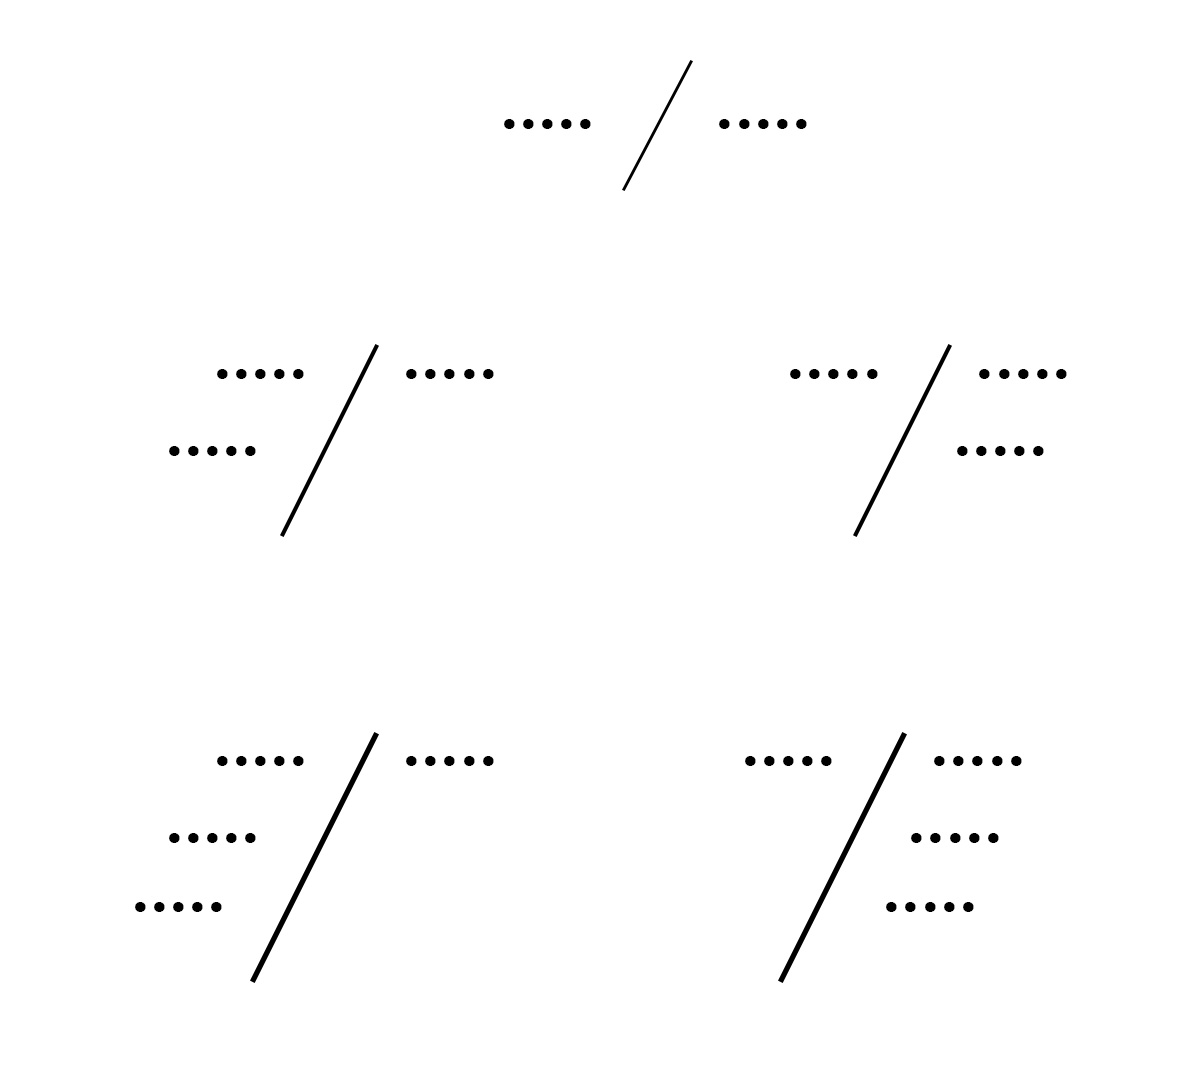
\includegraphics[height=5cm]{images/bs_types}
	\caption[Buchungssatzarten]{Grundformen der Buchungssätze.}
\end{figure}
  
\noindent ,,Zur schnellen und klaren Formulierung einer Buchung verwendet man den \textbf{Buchungssatz}. Der Buchungssatz besteht aus dem \textbf{Namen des Sollkontos}, dem Wort \textbf{,,an''} und dem \textbf{Namen des Habenkontos}''. (Haberl 2014, S. 174\nocite{RW1}) Die Sollseite befindet sich links von der Trennlinie und die Habenseite rechts.(vgl. ebda., S. 174\nocite{RW1}) Man unterscheidet zwischen zwei Kontoarten: \\

\subsubsection{Bestandskonten:}
,,Sie werden in \textbf{aktive} und \textbf{passive Bestandskonten} gegliedert.'' (ebda., S. 171\nocite{RW1}) Bei einem aktiven Bestandskonto wird eine Vermehrung auf der Sollseite verbucht und eine Verminderung auf der Habenseite. Bei passiven Bestandskonto ist es genau umgekehrt. (vgl. ebda., S. 184\nocite{RW1}) \\\\
Beispiele für aktive Bestandskonten: Bank, Vorsteuer, Kassa und Lieferforderungen und so weiter.
Beispiele für passive Bestandskonten: Umsatzsteuer, Lieferverbindlichkeiten und so weiter. (vgl. ebda., S. 173\nocite{RW1})

\subsubsection{Erfolgskonten:}
,,Konten, auf denen Geschäftsfälle erfasst werden, die \textbf{das Eigenkapital verändern}, werden als \textbf{Erfolgskonten} bezeichnet.'' (ebda., S. 186\nocite{RW1})
,,Erfolgskonten werden in \textbf{Aufwandskonten} und \textbf{Ertragskonten} gegliedert.'' (ebda., S. 187\nocite{RW1})
Bei einem Aufwandskonto wird eine Vermehrung auf der Sollseite verbucht und eine Verminderung auf der Habenseite. Bei Ertragskonten ist es genau umgekehrt. (vgl. ebda., S. 188\nocite{RW1})

\subsubsection{Steuern:}
\begin{itemize}
	\item Vorsteuer (2500):
	      ,,Auf diesem Konto wird die von den Lieferanten in Rechnung gestellte Vorsteuer verbucht.
	      Es ist [...] somit ein \textbf{aktives Bestandskonto}.'' (ebda., S. 248\nocite{RW1}) Wenn also etwas gekauft wird, nimmt die Vorsteuer zu und wird deshalb auf der Sollseite verbucht.
	\item Umsatzsteuer (3500):
	      ,,Dieses Konto dient zur Erfassung der Umsatzsteuer, die den Kunden in Rechnung gestellt wird.
	      Es ist [...] somit ein \textbf{passives Bestandskonto}.'' (ebda., S. 248\nocite{RW1}) Wenn also etwas verkauft wird, nimmt die Umsatzsteuer zu und wird deshalb auf der Habenseite verbucht.
\end{itemize}



\noindent So entsteht ein zweistufiger Buchungssatz. Einstufig ist er dann, wenn es sich um zwei Bestandskonten handelt. Dann spielen Steuern keine Rolle. Ein mehrstufiger Aufbau kommt zu Stande, wenn noch ein ,,Extrakonto'' für die Verbuchung benötigt wird. Diese Buchungssätze kommen jedoch verhältnismäßig selten vor.

\subsection{Berechnung der Beträge}
Bei einem einstufigen Buchungssatz gibt es nur einen Preis. Es ist abhängig von der Situation, ob dieser netto oder brutto hinzuschreiben ist. Ist eine Steuer involviert, gibt es mindestens drei Beträge, die den zugehörigen Konten zugeordnet werden. (vgl. ebda., S. 249\nocite{RW1}) Eventuell muss der Betrag des Extrakontos auch in die Berechnung des Prozentwertes miteinbezogen werden. Diese Faktoren summiert, bilden dann den Bruttobetrag, der auf der gegenüberliegenden Seite angeschrieben wird.
 

\section{Abschreibungen}
,,Unter \textbf{Anlagevermögen} versteht man alle \textbf{Wirtschaftsgüter}, die bestimmt sind, \textbf{dauernd} (länger als ein Jahr) \textbf{dem Geschäftsbetrieb zu dienen}, wie Grundstücke, Gebäude, Maschinen.'' (Haberl 2017, S. 32\nocite{RW4}) ,,Beim \textbf{abnutzbaren Anlagevermögen} sind die sich während der Nutzungsdauer ergebenden \textbf{Wertminderungen in Form von Abschreibungen} zu berücksichtigen.'' (ebda., S. 33\nocite{RW4}) Um den Betrag, der vom bisherigen Wert abgezogen wird, berechnen zu können, benötigt man folgende Informationen:
\begin{itemize}
	\item Anschaffungswert: ,,Der \textbf{Anschaffungswert} umfasst jene \textbf{Ausgaben}, die geleistet werden, um einen \textbf{Vermögensgegenstand zu erwerben} und \textbf{betriebsbereit} zu machen. Zum Anschaffungswert gehören auch die \textbf{Nebenkosten; Preisminderungen} sind abzuziehen.'' (ebda., S. 32\nocite{RW4})
	\item Nutzungsdauer: ist fix festgelegt
	\item Datum der Inbetriebnahme
\end{itemize}

\subsection{Ganzjahres- und halbjahres-AfA}
Es wird außerdem zwischen einer ,,ganzjahres-AfA'' und einer ,,halbjahres-AfA'' unterschieden. ,,Wird das Anlagegut \textbf{in der ersten Jahreshälfte in Betrieb genommen}, ist die \textbf{gesamte Jahresabschreibung} zu berücksichtigen. Erfolgt die \textbf{Inbetriebnahme} in der \textbf{zweiten Jahreshälfte des Geschäftsjahres}, ist die \textbf{Hälfte der Jahresabschreibung} anzusetzen.'' (ebda., S. 34\nocite{RW4})
Es wird also nur halb so viel abgenutzt und deshalb halbiert man auch den abzuschreibenden Betrag. Da zum Schluss noch ein halbes Jahr zum Abschreiben übrig bleibt, dauert der Abschreibungsprozess einer halbjahres-AfA ein Jahr länger. Es ergibt sich folgende Formel:


\begin{equation}
	Abschreibungsbetrag = \frac{Anschaffungswert}{Nutzungsdauer}
\end{equation} (vgl. ebda., S. 35\nocite{RW4})

\subsection{Erinnerungseuro}
,,Verbleibt die Anlage \textbf{nach dem Ende der Nutzungsdauer weiterhin im Betrieb}, erfolgt eine Abschreibung auf den \textbf{Erinnerungseuro}. Dabei wird der \textbf{Abschreibungsbetrag des letzten Jahres} der Nutzungsdauer \textbf{um einen Euro gekürzt}. Der Erinnerungseuro bleibt \textbf{solange in der Buchführung} stehen, \textbf{bis die Anlage ausscheidet}. Dann wird auch der Erinnerungseuro abgeschrieben.'' (ebda., S. 34\nocite{RW4})

\section{Identitätspreisverfahren}

Im Zuge der Inventur werden am Jahresende die Warenbestände im Unternehmen protokolliert. Ein wichtiges Verfahren ist dabei das Identitätspreisverfahren. Um diese Rechnung zu verstehen, müssen aber vorerst einige Begriffe geklärt werden:

\begin{itemize}
	\item Abfassungen: Das sind Waren, die im Laufe des Jahres aus dem Unternehmen ausgeschieden sind. Zum Beispiel durch einen Verkauf oder aufgrund eines Schadensfalles und so weiter.
	\item Soll-Endbestand: Bestand, der laut Lagerbuchführung bei der Inventur eigentlich ermittelt werden sollte.
	\item Schwund: Verlust von Waren durch zum Beispiel Beschädigung, Diebstahl oder Preisrückgang (vgl. ebda., S. 81\nocite{RW4})
	\item Ist-Endbestand: Bestand, der bei der Inventur tatsächlich ermittelt wird. Soll-Endbestand - Schwund. (vgl. ebda., S. 81\nocite{RW4})
	\item Niederstwertprinzip: ,,Ist der \textbf{Preis am Abschlussstichtag niedriger als der jeweilige Einstandspreis} [...], ist entsprechend [...] der \textbf{niedrigere Preis am Abschlussstichtag anzusetzen} [...].'' (ebda., S. 94\nocite{RW4})
	\item Abwertung: So kann es zu einer Abwertung des Anlagegutes kommen, die bei dem Identitätspreisverfahren, wie wir gleich sehen werden, auch eine Rolle spielt.
\end{itemize}

\noindent Beim Identitätspreisverfahren werden zuerst alle Zukäufe und der Anfangsbestand zusammengezählt und davon alle Abfassungen subtrahiert. Die Summe der Abfassungen wird auch als Wareneinsatz bezeichnet. Die Differenz zwischen diesen beiden Beträgen ergibt dann den Soll-Endbestand. Der Ist-Endbestand ist angegeben und die Differenz zwischen dem Soll-Endbestand und diesem ist der Schwund. Für den Bilanzansatz müssen dann die übriggebliebenen Waren bewertet werden. Ist der aktuelle Preis niedriger als der alte, muss abgewertet werden. Um die gesamte Abwertung herauszubekommen, muss der neue Verkaufspreis jeder Ware, von dem alten subtrahiert werden. Die Summe dieser Subtraktionen ergibt die Abwertung. (vgl. ebda., S. 87\nocite{RW4})

\noindent Die Ergebnisse werden schließlich mit zwei Buchungssätzen festgehalten:
\[ 7800 / 5010\text{                                      }\text{                                      }\text{                                      }\text{                                      }(Abwertung + Schwund) \]
Dann wird der Anfangsbestand vom Bilanzansatz (Endbestand) subtrahiert, um die Bestandsverminderung beziehungsweise die Bestandsvermehrung zu berechnen. Ist die Differenz negativ, bedeutet das, dass sich der Bestand im Vergleich zum Vorjahr vermindert hat. Ist sie positiv, hat er sich vermehrt. o. B. d. A. nehmen wir an, dass eine Bestandsvermehrung stattgefunden hat. Andernfalls würde der folgende Buchungssatz umgedreht werden.
\[ 1600 / 5010\text{                                      }\text{                                      }\text{                                      }\text{                                      }|Endbestand - Anfangsbestand| \]  (vgl. ebda., S. 87\nocite{RW4})



 
 
\chapter{Code-technische Umsetzung}
\rhead{KAPITEL 5.  CODE-TECHNISCHE UMSETZUNG}
  
Folgende Funktionen befinden sich im Paket Model in der Klasse MainModel.
 
\section{Grundformen der Buchungssätze}
Wie im Rechnungswesen-Abschnitt schon erklärt wurde, kommen Buchungssätze grundsätzlich in drei Grundformen vor. Hierbei wird die Umkehrung nicht mit einberechnet. Jede dieser Formen erfordert aufgrund der unterschiedlichen Berechnung eine gesonderte Behandlung.
 
\subsection{Einstufige Buchungssätze}
Diese können am einfachsten gehandhabt werden. Die Konten sind auf einer Ebene, genau so wie der Preis. Bei der Umkehrung müssen nur die beiden Konten vertauscht werden, wobei der Preis an Ort und Stelle bleibt. Zudem muss nur von netto auf brutto und umgekehrt gerechnet werden. Dies wird durch folgende Funktion implementiert.
 
 
\begin{lstlisting}
nettoToBrutto(String percent, String price)
\end{lstlisting}
	
\noindent Diese Funktion ruft nach abgeschlossener Berechnung eine weitere Funktion auf, welche die Ergebnisse auf die Benutzeroberfläche schreibt. Dazu gibt es natürlich auch eine Version, die von brutto auf netto rechnet.
 
\subsection{Zweistufige Buchungssätze}
Diese Form bringt ein zusätzliches Konto mit sich, nämlich die Steuer. So muss diese jetzt auch immer ausgerechnet werden. Das führt vermehrt zu Rundungsfehlern, welche in einer separaten Methode möglichst klein gehalten werden. Auch verändert sich das Konto bei der Umkehrung. 

\subsection{Mehrstufige Buchungssätze}
Ein neues Konto, das nicht, wie bei der Steuer, eindeutig festgelegt ist, ergänzt die bisher verwendeten Konten. So muss nun eine neue Komponente, ein Textfeld, in die Benutzeroberfläche eingebaut werden, um es dem User zu ermöglichen, selbstständig Werte einzugeben. Neben dem Feld für den Preis, gibt es nun auch ein Feld für den Betrag des Extrakontos. Um den Bruttobetrag zu berechnen, muss jetzt der Betrag des ersten Aufwandskontos zu dem des zweiten addiert und davon 20 Prozent ausgerechnet werden. Diese werden dann zur Summe addiert und dieser Betrag ergibt dann den Bruttobetrag. Die Berechnung der anderen Beträge, können vom Leser selbst erschlossen werden.

\begin{lstlisting}
Double[] nettoToBrutto(String nettoPrice, String otherPrice, String percent)
\end{lstlisting}

\noindent Auch hier gibt es wieder eine Version, die von brutto auf netto rechnet.

\section{Ausnahmefälle}
Die Ausnahmefälle sind wie immer diejenigen, welche am schwierigsten zu behandeln sind. Sie lassen sich grundsätzlich auf die Grundformen zurückführen, jedoch erfordern die kleinen Veränderungen oft neue GUI-Elemente und Algorithmen. Besonders Themen wie die Berechnung des Tagesgeldes oder das Abschreiben, erfordern neue Lösungen und komplett andere Benutzeroberflächen, wegen der zusätzlichen Parameter, die zur Berechnung benötigt werden. Auf letztere wird nun gesondert eingegangen.


\subsection{Methode für das Abschreiben}
  
\begin{lstlisting}
calcAbschreibung(String anlKonto, String IBN_Monat_str, String IBN_Year, String ND_str, Double AW, String command)
\end{lstlisting}
Zuerst werden natürlich alle benötigten Argumente geholt: Anlagenkonto, Monat der Inbetriebnahme, Jahr der Inbetriebnahme, Nutzungsdauer, Anschaffungswert, command. Der command enthält einen String, der signalisiert wie viele Abschreibungen angezeigt werden sollen. Es gibt vier Optionen: alle Jahre, erste zwei Jahre, letzte zwei Jahre und erstes Jahr. All diese Faktoren müssen selbstverständlich auch mit GUI-Bausteinen auf der Benutzeroberfläche abgebildet werden.
Für den weiteren Codeverlauf ist wichtig zu wissen, dass einige globale Variablen erstellt wurden:\\

\begin{itemize}
	\item String tempYear wird für die ,,getDate''-Methode gebraucht
	\item private static LinkedList<String> llYear: Hier werden die abgeschriebenen Jahre gespeichert
	\item private static LinkedList<Double> llAfaPrice: Hier werden die abgeschriebenen Beträge gespeichert
\end{itemize}


\begin{lstlisting}
		
	tempYear = IBN_Year;
		
	Double nd = Double.parseDouble(ND_str);
	int IBN_Monat = Integer.parseInt(IBN_Monat_str);
	
	Double afaBetrag = AW/nd;
	
	llYear.addLast(tempYear);
	
\end{lstlisting}
Es finden einige Typ-Umwandlungen statt und der AfA-Betrag wird standardmäßig berechnet. Das aktuelle Jahr wird abgespeichert.\\

\begin{lstlisting}
					
	for(int x = 0; x < nd-1; x++) {
		llYear.addLast(getDate());
		llAfaPrice.addLast(afaBetrag);
	}
	
	llAfaPrice.set(llAfaPrice.size()-1, afaBetrag-1);
	
	if(IBN_Monat > 6) {
		llAfaPrice.set(0, afaBetrag/2);
		llAfaPrice.set(llAfaPrice.size()-1, afaBetrag);
		llAfaPrice.addLast(afaBetrag/2-1);
		llYear.addLast(getDate());
		afaBetrag = afaBetrag/2;
		
\end{lstlisting}

\noindent Anschließend werden in einer Schleife die Daten inkrementiert und der AfA-Betrag, der bei einer ganzjahres-AfA immer gleich bleibt, zu den zwei Listen hinzugefügt.  Da im letzten Abschreibungsjahr ein ,,Erinnerungseuro'' übrig bleibt, wird der AfA-Betrag - 1 hinzugefügt. Da eine halbjahres-AfA bis auf den ersten und letzten Betrag und der Länge identisch zu einer g.j-AfA ist. Wurde zuerst der Prozess der g.j.-AfA vollzogen. Jetzt wird überprüft, ob es sich um eine h.j.-AfA handelt. Wenn ja, wird der erste Betrag standardmäßig halbiert und der momentan letzte Betrag, der ja vorher wegen dem Erinnerungseuro - 1 genommen wurde, inkrementiert. Dann wird ein weiterer Eintrag hinzugefügt, der nun der letzte Betrag ist und deshalb halbiert und dekrementiert werden muss. Der AfA-Betrag einer h.j.-AfA wird für weitere Berechnungen angepasst.
	
\begin{lstlisting}
		
	if(command.equals("erste zwei Jahre"))
	    addAfAToPanel(0, 1, anlKonto);
	
	else if(command.equals("letzte zwei Jahre"))
	    addAfAToPanel(llAfaPrice.size()-2, llAfaPrice.size()-1, anlKonto);
	
	else if(command.equals("alle Jahre"))
	    addAfAToPanel(0, llAfaPrice.size()-1, anlKonto);
	
	else if(command.equals("erstes Jahr"))
	    addAfAToPanel(0, 0, anlKonto);
	
	llAfaPrice.removeAll(llAfaPrice);
	llYear.removeAll(llYear);
	
	return afaBetrag;
}
\end{lstlisting}

\noindent Nun wird auf Grundlage des commands entschieden, wie viele ausgegebene Abschreibungen vom User erwünscht sind. Diese werden dann aus den Listen herausgefiltert und mittels der Methode ,,addAfAToPanel'' auf der Benutzeroberfläche abgebildet.
  
\section{Kalkulationen}
Kalkulationen sind die einfachsten und vorhersehbarsten Berechnungen im Programm. Sie folgen immer dem gleichen Schema und deshalb muss, anders als bei den Buchungssätzen, verhältnismäßig wenig Code für Abweichungen geschrieben werden. Es gibt jedoch auch hier eine Umkehrung, die gesondert behandelt werden muss. Es gibt außerdem eine Funktion, die einen gewissen Grad an Multitasking erlaubt. Ist man mit einer Kalkulation noch nicht fertig oder will man sie derzeit nicht löschen, klickt man einfach eine andere an. Im Menü ,,Kalkulationen'' erscheint dann die Anzahl der offenen Kalkulationen. Wechselt man wieder zur alten, kann man diese löschen und der Counter wird dekrementiert. So ist man nicht auf eine beschränkt.
\subsection{Gehalts- und Lohnverrechnung}
Eine weitere Kalkulation, die einem festgelegten Schema folgt. Sie unterscheidet sich jedoch von den anderen Kalkulationen, aufgrund der regelmäßigen Veränderungen, bezüglich der Prozentsätze. Diese ändern sich jährlich und deshalb wurde eine Funktion eingebaut, die es dem Nutzer erlaubt, selbstständig die Daten auf dem neuesten Stand zu halten. Diese werden extern in einer Textdatei gespeichert und ein- beziehungsweise ausgelesen. Außerdem wird der User aufgefordert, selbst Daten aus einer Tabelle herauszulesen, um die Implementation dieser vorzubeugen.





\chapter{Benutzeroberfläche}
\rhead{KAPITEL 6.  BENUTZEROBERFLÄCHE}
 
In diesem Kapitel werden die einzelnen Ansichten und die, vom User sichtbaren, Komponenten und Funktionen erklärt.
 
\section{Hauptarbeitsflächen}
Die Buchungssatz- und Kalkulationsansicht des Programms besteht grundsätzlich aus drei Hauptarbeitsflächen. Auf der linken Seite befindet sich das Hauptmenü. Dort sind untereinander alle aufgegriffenen Kapitel angeordnet. Nachdem eines angeklickt wurde öffnet sich eine weitere Auflistung in der Mitte. Dort sind dann alle Buchungssätze oder Kalkulationen, die im Kapitel vorkommen zu finden. Nach der Auswahl eines dieser öffnet sich das erste Fenster, in welchem eine kleine Vorschau des Buchungssatzes und Eingabefelder für den Benutzer erscheinen. Wird der Bestätigen-Button gedrückt, wird der fertig ausgerechnete Buchungssatz auf der Hauptarbeitsfläche auf der rechten Seite abgebildet. Da die Lösung einer Kalkulation viel mehr Platz beansprucht, wird diese auf der Arbeitsfläche in der Mitte ausgegeben. Gleichzeitig erscheint beim Kapitel ,,Kalkulationen'' die Zahl der aktiven Kalkulationen. Wird eine weitere geöffnet inkrementiert auch diese Zahl.

\begin{figure}[h]
	\centering
	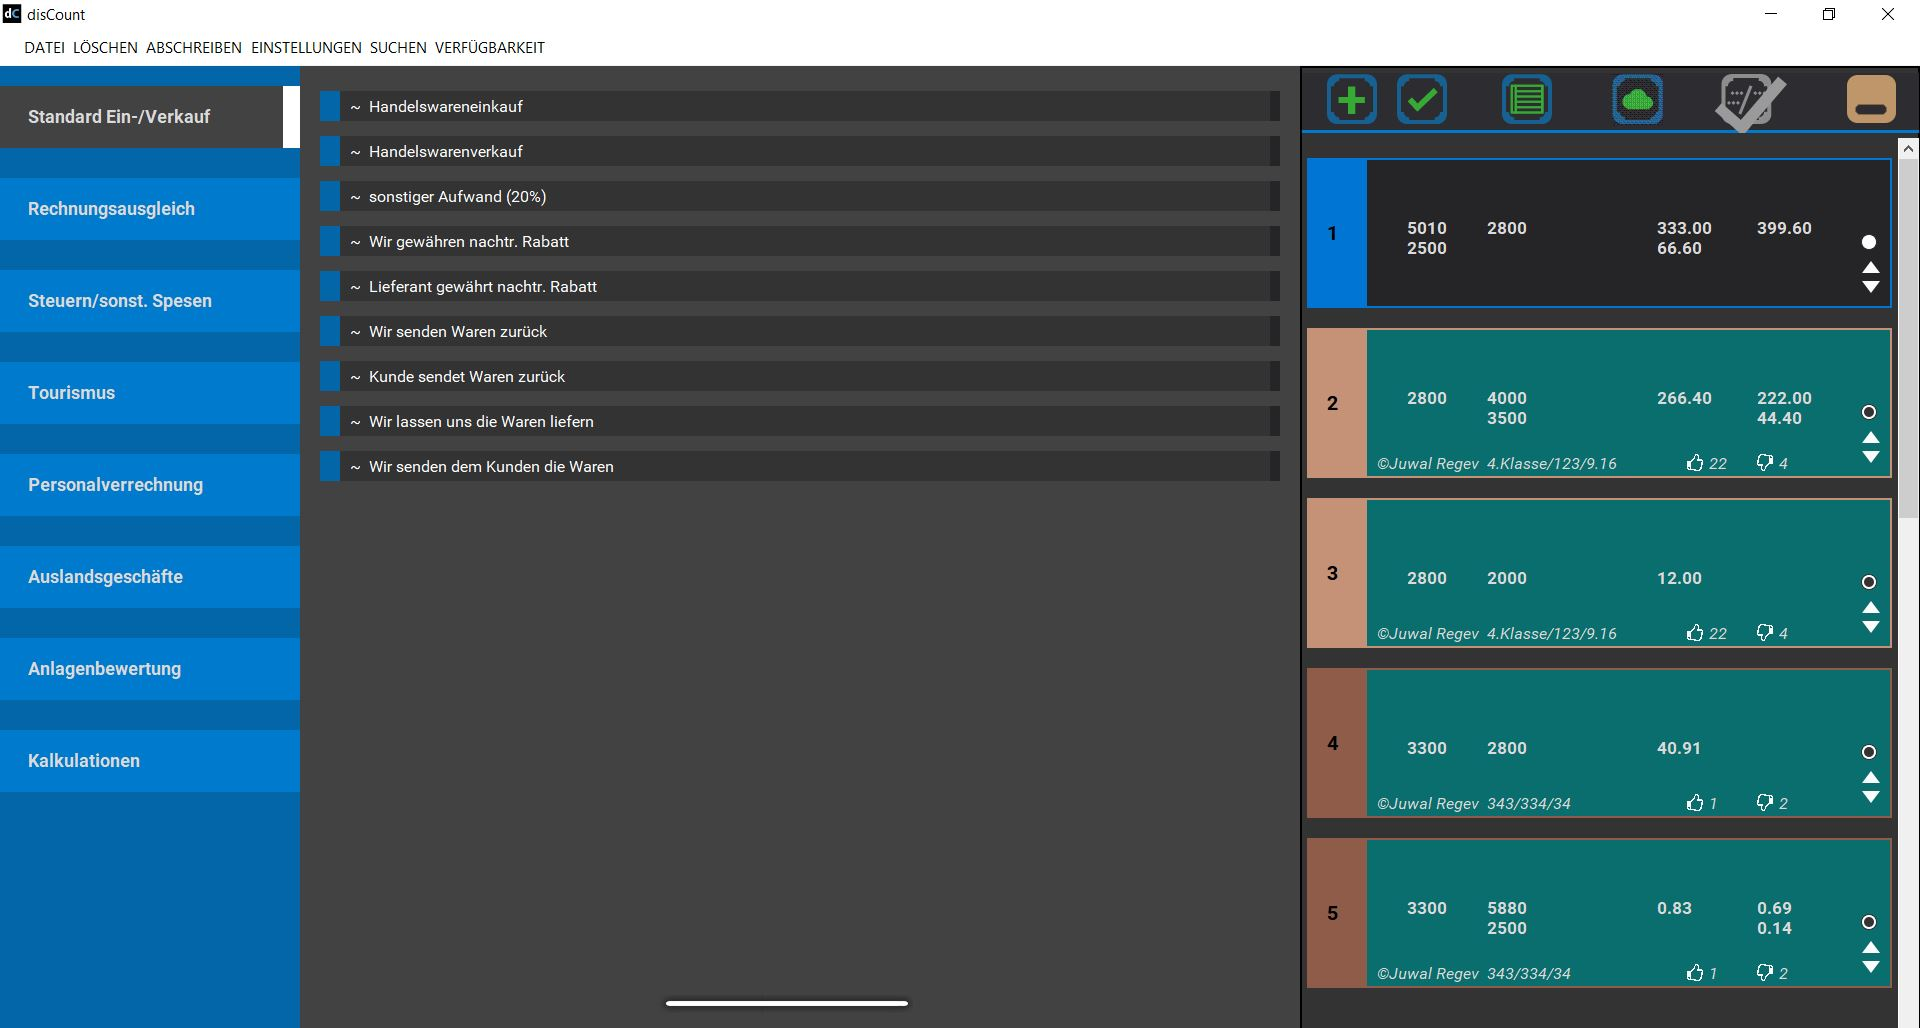
\includegraphics[height=7cm]{images/hauptarbeitsflaechen}
	\caption[Hauptarbeitsflächen]{Die drei Hauptarbeitsflächen in disCount.}
\end{figure}


\subsection{Menü}
Wie bei den meisten Programmen ist das Menü ganz oben angeordnet. Es enthält die Registerkarten ,,Datei'', ,,Löschen'', ,,Abschreiben'', ,,Einstellungen'' und ,,Suchen''. Viele dieser Funktionen sind auch durch Shortcuts erreichbar. Die meisten Funktionen, die im Menü enthalten sind, sind selbsterklärend und deshalb werden wir nur auf die zwei wichtigsten eingehen. Die Kategorie ,,Abschreiben'', wird im Zuge des Erläuterns der elementare Funktionen behandelt.

\subsubsection{Einstellungen}
Das Untermenü dieser Registerkarte enthält Funktionen zum Ändern der Grundeinstellung der Personalverrechnung. Da sich dort die Prozentsätze jährlich ändern und ,,disCount'' keine Updates unterstützt, kann man in dem Einstellungsmenü selbstständig diese Daten ändern.

\begin{figure}[h]
	\centering
	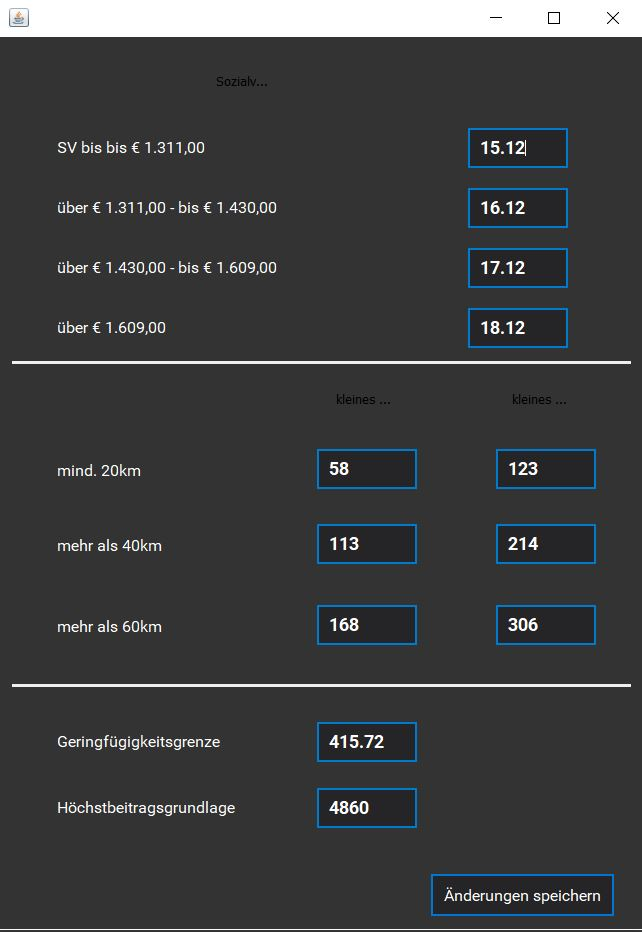
\includegraphics[height=13cm]{images/einstellungen}
	\caption[Einstellungen]{Grundeinstellung der Personalverrechnung.}
\end{figure}

\subsubsection{Suchen}
Damit der Benutzer so schnell wie möglich zum gewünschten Buchungssatz kommt, gibt es die Suchfunktion. Das Suchfenster besteht aus einer Suchleiste und einem Bereich, in welchem die Ergebnisse angezeigt werden. Abgesehen vom Namen des Buchungssatzes, wird auch der Pfad angezeigt. Im Kapitel !!! wird die Suchfunktion genauer erläutert.

\begin{figure}[h]
	\centering
	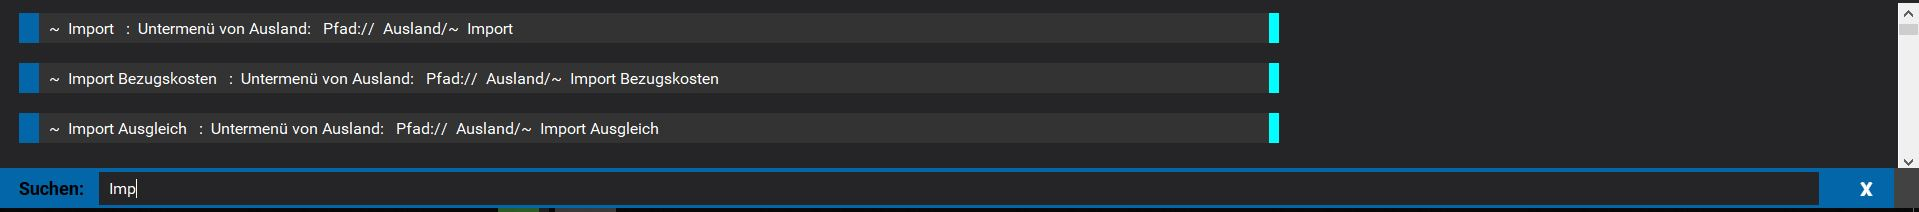
\includegraphics[width=16cm]{images/suchen}
	\caption[Suchen]{Suchen in disCount.}
\end{figure}

\section{Unterstützung kleiner Bildschirmauflösungen}
Im Programm wird das in JAVA eingebaute ,,BorderLayout'' verwendet. Dieses besteht aus einer Nord-, Ost-, Süd- und Westseite, die auch bis auf die Nordseite benutzt werden. Ein tolle Funktion vom BorderLayout ist, dass es sich beim Verkleinern des Fensters automatisch anpasst. Speziell bei den Kalkulationen verdeckt das Ostpanel aber schnell den Inhalt. Deshalb kann man durch ein Wischen über ein Viereck auf dem Ostpanel, dieses einklappen, um einen größeren Arbeitsbereich zu erhalten. Es wurde auch eine Funktion für schnelles Suchen eingebaut. Dazu gibt es am unteren Rand des mittleren Panels eine weiße Leiste, die beim Darüberstreichen die Suche ausklappt und wieder einklappt.


\part{Datenbank}


\chapter{Lösungsvorschläge}
\rhead{KAPITEL 8.  LÖSUNGSVORSCHLÄGE}
 
Richtige Lösungen sind für effizientes Üben sehr wichtig. Auch können Sie sehr hilfreich sein, wenn man einmal nicht weiterkommt. Deshalb wurde ein System entwickelt, das bei Bedarf einen möglichen Lösungsweg vorschlägt.

\section{Zielsetzung}
Das System soll in der Lage sein, fertige Aufgaben von Benutzerinnen und Benutzern aufzunehmen und diese bei identischem Lösungsanfang vorzuschlagen. Die Schülerinnen und Schüler müssen sich dabei bei der Einsendung der Lösung sicher sein, dass diese korrekt ist und die Aufgabe auch im Schulbuch existiert. Der Lösungsvorschlag soll Informationen über den Einsender sowie über die Lösung selbst, wie Schulbuch, Seite und Nummer haben. Außerdem soll die Vertrauenswürdigkeit des Hochladers klar ersichtlich sein. So wird eine Lösung, die von einer Lehrperson hochgeladen wurde, mit einem Stern markiert und Lösungen von SchülerInnen, welche mehr als fünf Likes erhalten haben, mit einem Verifikation-Häkchen dargestellt. Es soll auch möglich sein, die Lösung mit einem Daumen nach oben beziehungsweise nach unten bewerten zu können und Kommentare zu verfassen. Lösungsvorschläge werden erst nach dem Hochladen von fünf Lösungen aktiviert. Dadurch soll die Bereitschaft zum Teilen von Lösungen angekurbelt werden.

\section{Funktionsweise}

\subsection{Datenbank}
Damit jeder Zugriff auf die gleichen Informationen hat, wird das Programm mit einer Datenbank verbunden. In einer der Tabellen werden dann die Informationen der Lösung gespeichert: Primärschlüssel, Name des Einsenders, Schulbuch, Seite und Nummer der Aufgabe, Anzahl der Daumen hoch beziehungsweise runter und vieles mehr.

\subsection{Einsendung}
Will die Nutzerin ihre oder der Nutzer seine Arbeit speichern, wird gefragt, ob sie oder er ihre oder seine Lösungen veröffentlichen möchte. Stimmt sie oder er zu, werden die Buchungssätze in eine später erläuterte Codierung umgewandelt und auf die Datenbank hochgeladen.

\subsection{Abfrage}
Die BenutzerInnen müssen explizit das Buch, die Seite und Nummer der von ihnen bearbeiteten Aufgabe eingeben. Dann können sie noch auswählen, dass nur Lehrerlösungen angezeigt werden sollen. Es wird dann nach Übereinstimmungen in der Datenbank gesucht. Grundsätzlich setzt sich die Lösung mit den meisten Daumen hoch durch. Eine Lehrerlösung hat jedoch immer Vorrang.

\subsection{Registrierung als LehrerIn}
Damit bei den Lösungsvorschlägen zwischen LehrerIn und SchülerIn unterschieden werden kann, muss es eine Möglichkeit geben, sich als LehrerIn zu registrieren. Am Anfang haben alle Accounts standardmäßig einen SchülerInnen-Status. Um LehrerInnen-Rechte zu erhalten, müssen  sich die Lehrpersonen an den Administrator wenden. Dazu genügt eine E-Mail, wobei das Verifikationsverfahren noch nicht bekannt ist. Ist bewiesen, dass es sich bei dem Anwärter auch wirklich um eine Lehrperson handelt, wird ein Code zur Verfügung gestellt. Diesen gibt er oder sie dann in das Fester ein, welches unter dem Menüpunkt ,,Lehrer'' - ,,Code anfordern'' erscheint. Gibt es eine Übereinstimmung mit der Datenbank, wechselt der SchülerInnen-Account in einen LehrerInnen-Account.   



\chapter{Fehlerkorrektur}
\rhead{KAPITEL 9.  FEHLERKORREKTUR}
 
Um selbstständig Üben zu können, sind richtige Lösungen zur Überprüfung essenziell.

\section{Zielsetzung}
Das System soll in der Lage sein, Buchungssätze auf ihre Korrektheit zu überprüfen. Es soll außerdem auf die Art des Fehlers hingewiesen werden. Diese Funktion wird ebenfalls erst nach dem Hochladen von fünf Lösungen aktiviert.

\section{Fehlererkennung}
Die zur Überprüfung eingereichte Aufgabe wird zuerst in ihre encodierte Form umgewandelt. Die richtige Lösung, ebenfalls in encodierter Form, wird dann von der Datenbank heruntergeladen und mit dem encodierten String verglichen. Zu erkennen, ob eine Fehler existiert ist dann trivial. Die Schwierigkeit liegt darin, die Art des Fehlers zu erkennen.

\subsection{Fehlende Buchungssätze}

\subsubsection{Problemstellung}
Angenommen in einem System werden die Buchungssätze nacheinander verglichen. Angenommen es fehlt ein Buchungssatz, jedoch alle anderen sind richtig. Es werden alle nachfolgenden Buchungssätze auch als falsch markiert, obwohl sie eigentlich richtig sind, da sie ja um eine Stelle verschoben sind. Ein solches Korrektursystem wäre für die Benutzerin oder den Benutzer nicht sehr hilfreich. Deshalb muss eine Funktion eingebaut werden, die diesen Vorfall erkennt und dann richtig handelt. 


\subsubsection{Lösung}
Zur Erklärung werden die in der darunterliegenden Abbildung dargestellten Elemente benutzt. Die Buchungssätze sind mit dem Kürzel zum Beispiel ,,F1'', das für ,,falscher Buchungssatz Nummer eins'' steht, benannt. Der Inhalt des Buchungssatzes wird mit einer Zahl dargestellt.\\
Aus der Abbildung kann man leicht herauslesen, dass in der falschen Lösung zwei Buchungssätze, nämlich R2 und R3, fehlen. Zuerst wird F1 mit R1 verglichen. Die zwei Buchungssätze stimmen überein. Dann wird F2 mit R2 verglichen. Es gibt keine Übereinstimmung und deshalb wird eine Methode ,,checkIfBSmissing'' aufgerufen. Das Ziel dieser Methode ist es, herauszufinden, ob es in der richtigen Lösung irgendwo einen Buchungssatz gibt, der mit F2 übereinstimmt. Da F2 und R2 nicht übereinstimmen, wird R2 in die Liste ,,wrongList'' eingetragen. Jetzt wird F2 mit R3 verglichen und wieder wird R3 in die Liste ,,wrongList'' eingetragen. Schließlich wird F2 mit R4 verglichen. Diese stimmen überein und somit lässt sich darauf schließen, dass R2 und R3 in der falschen Lösung ,,nur'' fehlen.\footnote{Es kommt praktisch nie vor, dass ein Buchungssatz in einer Aufgabe zweimal vorkommt.} R2 und R3 werden also als falsch markiert, R4 als richtig. Außerdem werden in der falschen Lösung zwischen F1 und F2 zwei Platzhalter hinzugefügt, um die Anzahl an Buchungssätzen in der falschen und richtigen Lösung auszugleichen, um so weitere Vergleiche möglich zu machen.\\Die Methode ,,checkIfBSmissing'' hat ihre Arbeit getan und kehrt zurück. Schließlich geht es mit dem Vergleich zwischen F3 und R5 weiter.

\begin{figure}[h]
	\centering
	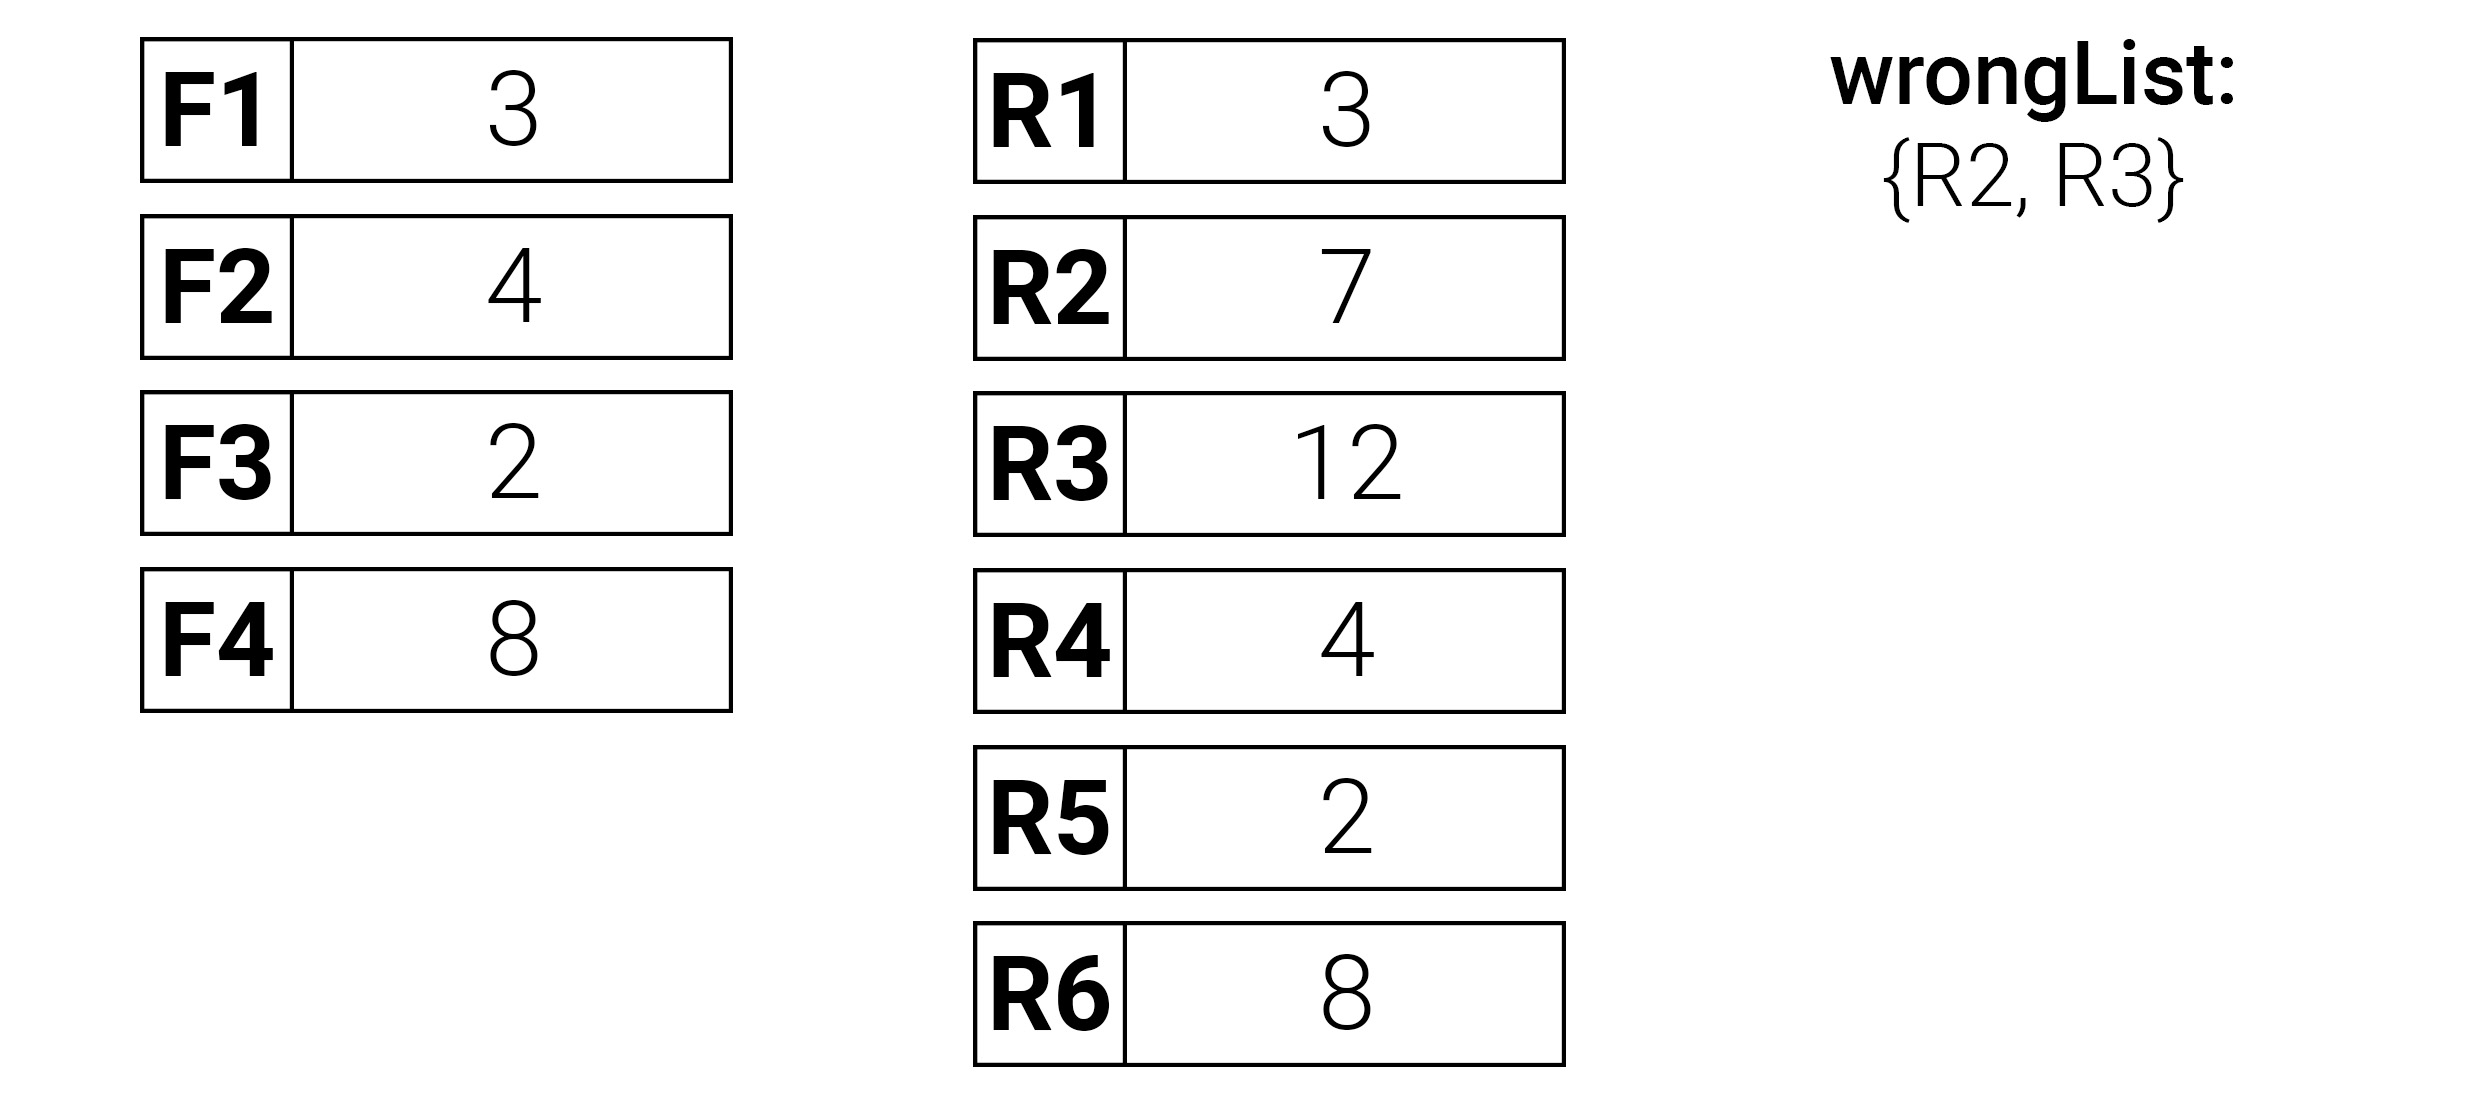
\includegraphics[height=5cm]{images/missingBS}
	\caption[Problem fehlende Buchungssätze]{Darstellung des Problems}
\end{figure}
  
  
\subsection{Zu viele Buchungssätze}
Der Algorithmus zur Erkennung zu vieler Buchungssätze operiert ähnlich zu dem gerade besprochenen.
 
\subsubsection{Lösung}
Aus der darunterliegenden Abbildung ist leicht zu erkennen, dass in der falschen Lösung F2 und F3 zu viel sind. Nachdem F1 und R1 verglichen wurden und bei F2 und R3 keine Übereinstimmung gefunden wurde, wird eine Methode ,,checkIfBSoverload'' aufgerufen. Das Ziel dieser Methode ist es, im Gegensatz zur oben besprochenen, herauszufinden, ob es in der \textbf{falschen} Lösung irgendwo einen Buchungssatz gibt, der mit \textbf{R2} übereinstimmt. Da F2 und R2 nicht übereinstimmen, wird F2 in die Liste ,,wrongList'' eingetragen. Jetzt wird R2 mit F3 verglichen und wieder wird F3 in die Liste ,,wrongList'' eingetragen. Schließlich wird R2 mit F4 verglichen. Diese stimmen überein und somit lässt sich darauf schließen, dass F2 und F3 in der falschen Lösung zu viel sind. R2 wird als richtig markiert, es wird jedoch eine Meldung ausgegeben, die darauf hinweist, dass darüber zwei Buchungssätze zu viel waren. F2 und F3 werden entfernt, um die Anzahl an Buchungssätzen in der falschen und richtigen Lösung auszugleichen, die Methode kehrt zurück und es geht weiter mit dem Vergleich zwischen F5 und R3.
 
 
\begin{figure}[h]
	\centering
	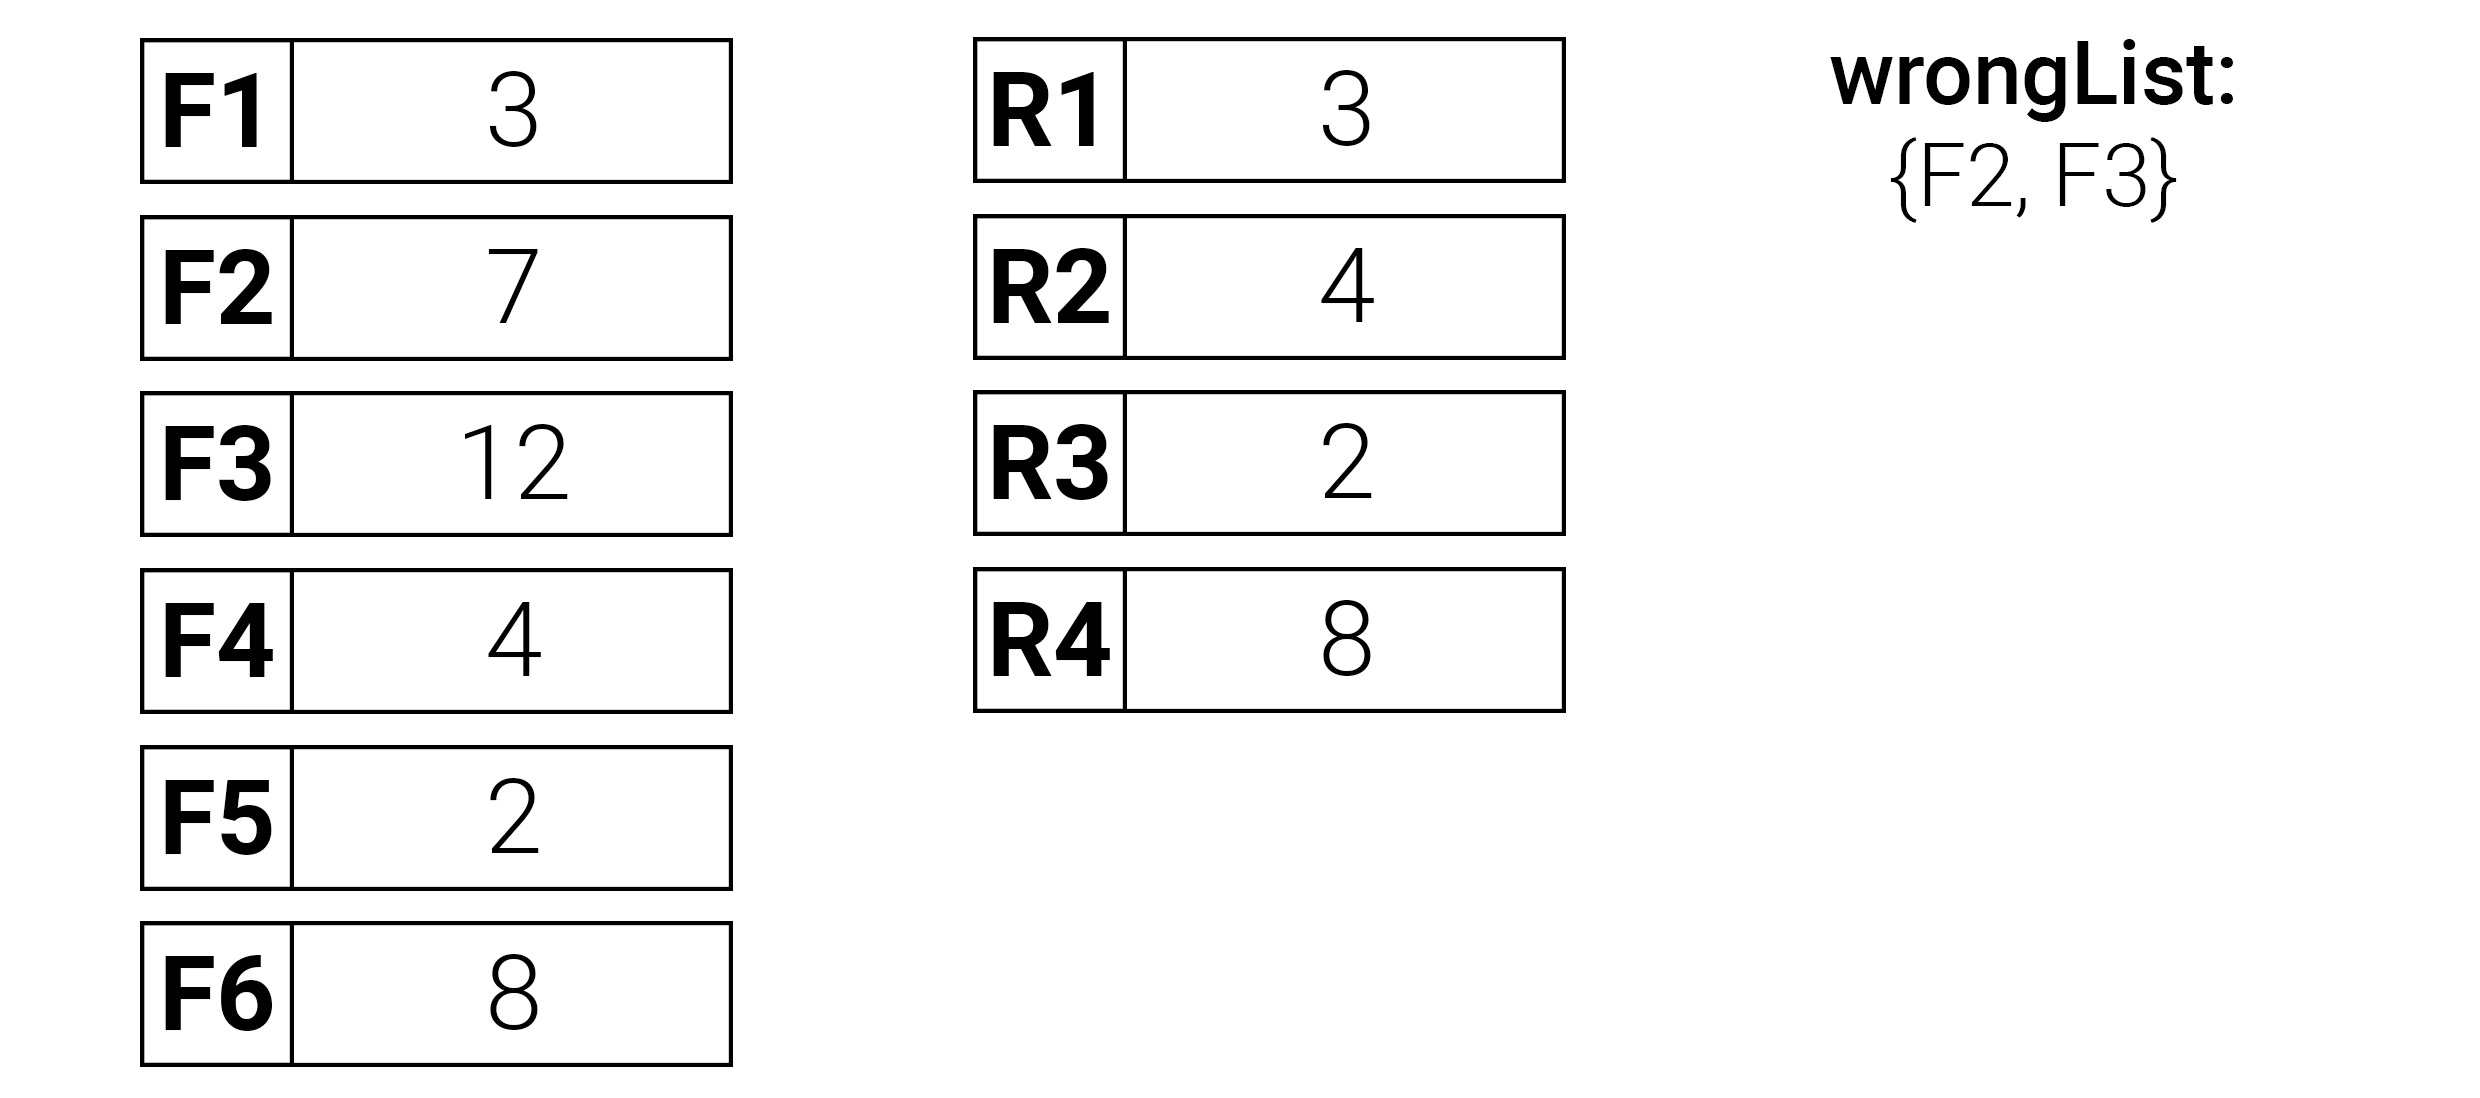
\includegraphics[height=5cm]{images/BSoverload}
	\caption[Problem zu viele Buchungssätze]{Darstellung des zweiten Problems}
\end{figure}
  
  
  
\chapter{Prüfungen}
\rhead{KAPITEL 9.  PRÜFUNGEN}
 
Auch hinsichtlich Prüfungen lässt sich im Rechnungswesen einiges optimieren.
 
\section{Ziel}
Prüfungen in disCount sollen die herkömmliche Prüfungsabwicklung nicht nur ersetzen, sondern auch erheblich verbessern. Speziell LehrerInnen sollen davon profitieren. Die Kontrolle soll komplett von der Software übernommen werden. Auch die Auswertung der Ergebnisse, auf welche die LehrerInnen häufig verzichten, wird durch das Programm erledigt. Außerdem soll das Schummeln unterbunden werden.
  
\section{Umsetzung}
Zuerst muss die Lehrperson die Lösung der Prüfung anhängen und die Anzahl an Teilnehmern angeben. Dann wird eine Prüfungsidentifikationsnummer vergeben. Die SchülerInnen gehen auf den Menüpunkt ,,Prüfung beitreten'' und geben diese PIN ein. Sie werden dann zum Warten aufgefordert. Die Lehrperson hat in der Zwischenzeit einen Überblick über alle beigetretenen SchülerInnen. Sind alle bereit, kann das Stagithugrtsignal vergeben werden und jegliche Funktionen wie Lösungsvorschläge oder Kommentare werden deaktiviert. Auch befinden sich die SchülerInnen ab der Erstellung des ersten Buchungssatzes in einer Prüfungsumgebung. Das heißt, dass diese während der Prüfung auch nicht mehr verlassen werden darf. Sollte das doch der Fall sein, wird der Schüler oder die Schülerin sofort aus der Prüfung geworfen und die Lehrerperson über das Vergehen informiert. 
  
\section{Funktionsweise Datenbank}
  
\subsection{Struktur}
  
Für das Speichern der Daten für Prüfungen, wurde eine eigene Tabelle ,,exams'' angelegt. Die Datensätze darin bestehen aus folgenden Attributen: \newline\newline \textbf{id, resultID, nextIn, pStart, solution, BShelp, student1, student2, student3, ..., bs1, bs2, bs3, ...} \newline\newline
  
\noindent Grundsätzlich gibt es in der Tabelle zwei Arten von Datensätzen: Den Prüfungsdatensatz und den Lösungsdatensatz. Sobald die Lehrperson eine neue Prüfung erstellt hat, werden diese zwei zur Tabelle hinzugefügt wobei in der resultID des Prüfungsdatensatzes die id des Lösungsdatensatzes gespeichert wird, um die Zusammengehörigkeit zu bewahren. In solution wird die Lehrerlösung eingetragen und in BShelp die Entscheidung der LehrerInnen, ob Computerunterstützung erlaubt ist. 

\subsection{Verbindung zur Prüfung}

Die Rechner der SchülerInnen verbinden sich dann mit der Datenbank und tragen ihre ID (von der Tabelle users) in die Spalte student... ein. Damit der Rechner weiß, welche Spalte bereits besetzt ist, wurde das Attribut nextIn eingeführt. Tragt sich der Schülercomputer in eine Spalte ein, die von nextIn angezeigt wird, inkrementiert er anschließend das Feld nextIn und somit kann nichts überschrieben werden.

\subsection{Prüfungsablauf}

Sobald sich alle TeilnehmerInnen eingetragen haben, kann die Lehrperson das Startsignal geben. Dieses wird im Feld pStart in Form eines Integers gespeichert. Die Prüfung ist somit gestartet. Wie bereits erwähnt wird der Lehrer sofort alarmiert, wenn ein Schüler oder eine Schülerin die Prüfungsumgebung verlässt.

\subsection{Prüfungsende, Ergebnis und Auswertung}

Ist ein Schüler oder eine Schülerin fertig, muss im Menü ,,Prüfung abgeben'' ausgewählt werden. Die Arbeit wird dann von disCount korrigiert. In eine Liste, welche zuvor mit Nullen gefüllt wurde, wird bei einem korrekten Buchungssatz eine Eins eingetragen. Also wenn zum Beispiel der dritte Buchungssatz richtig ist, wird beim Index drei eine Eins eingetragen. Somit lässt sich der Prozentsatz sehr leicht ausrechnen. In den dazugehörigen Lösungsdatensatz wird in die entsprechende Spalte (student...) dieser Prozentsatz eingetragen. Somit ist eindeutig ermittelbar, welcher Schüler beziehungsweise welche Schülerin welchen Prozentsatz erreicht hat. Zusätzlich wird noch die Erfolgsquote bei jedem Buchungssatz erfasst, damit die LehrerInnen nach Prüfungsschluss eine genaue Auswertung der Prüfung bekommen. Dafür gibt es im Lösungsdatensatz die Attribute ,,bs1, bs2, bs3, ...''. Dabei erfasst bs1 die Punkte, welche die TeilnehmerInnen insgesamt beim Buchungssatz eins erzielt haben und bs2 die Punkte bei Buchungssatz zwei und so weiter. Gibt der Schüler oder die Schülerin die Prüfung ab, wird also nicht nur der Prozentsatz gespeichert, sondern auch die Spalten bs1, bs2, bs3, ... werden entsprechend erhöht oder bleiben bei Misserfolg gleich. 

  

\part{disCount Verwaltungsprogramm}

\chapter{Ziel und Befehle}

\section{Ziel}
Um die Datensätze in der oben vorgestellten Datenbank einfach verwalten zu können, soll ein Konsolenprogramm geschrieben werden, welches Aufgaben wie das Ausgeben und Löschen von redundanten Lösungen und das Schreiben und Anzeigen von gelesenen Mitteilungen erledigt. Ansonsten müsste das mit einer grafischen Webanwendung, wie beispielsweise phpmyadmin gemacht werden. Bei vielen Datensätzen kann jedoch speziell das Suchen nach Dubletten in einer Spalte sehr mühsam bis nicht machbar sein. Das Programm soll wie bereits erwähnt von einer Konsole aus also mit Befehlen bedienbar sein. Deshalb soll es auch in der Programmiersprache C geschrieben werden und auf dem Linux-Betriebssystem laufen können.

\section{Befehle}

\subsection{Redundanzen}

\subsubsection{showDuplicates -hbla}
Manuell kann das Suchen nach Redundanzen sehr mühsam sein. Das Verwaltungsprogramm zeigt nach der Eingabe dieses Befehls den gesamten Datensatz aller identischen Lösungen, die in der Tabelle ,,usersolutionshbla'' an. Anstelle von ,,-hbla'' kann auch ein anderer Schultyp geschrieben werden.

\begin{figure}[h]
	\centering
	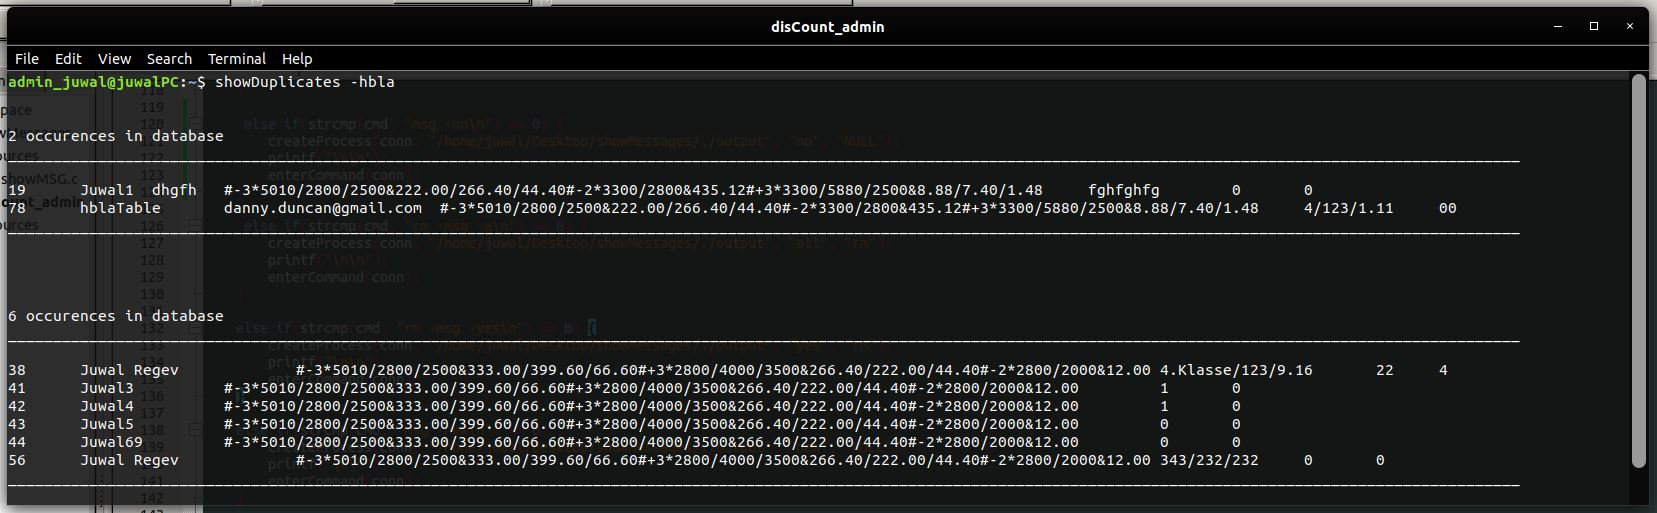
\includegraphics[width=15cm]{images/showDuplicates_hbla}
	\caption[Befehl showDuplicates -hbla]{Ergebnis des Befehls showDuplicates -hbla}
\end{figure}


\subsubsection{rm -hbla -a}
Dieser Befehl zeigt zuerst alle Redundanzen an und entfernt diese dann aus der Tabelle. Danach muss jedoch auch noch die Anzahl an hochgeladenen Lösungen der Nutzer und Nutzerinnen, deren Lösung entfernt wurde, um eins dekrementiert werden. Es kann hierbei natürlich vorkommen, dass ein Benutzer oder eine Benutzerin wieder unter die Grenze von fünf Beträgen kommt. Auch hier kann statt ,,hbla'' wieder ein anderer Schultyp eingesetzt werden.

\subsection{Nachrichten}

\subsubsection{msg -a}
Wenn der Administrator in disCount eine Nachricht an einen bestimmten Nutzer oder eine bestimmte Nutzerin senden will, kann er das mithilfe der Datenbank machen. In der Tabelle ..messages'' kann ein Empfänger oder eine Empfängerin, zwei Überschriften, der Inhalt und der Typ der Nachricht eingegeben werden. Beim nächsten Start von disCount holt sich das Programm die Nachricht von der Datenbank und blendet diese dann auf dem Bildschirm aus. Dann trägt das Programm in der Tabelle in der Spalte ,,received'' ,,yes'' ein und die Nachricht wird nicht wieder angezeigt. Der Befehl ,,msg -a'' zeigt alle Nachrichten an.

\begin{figure}[h]
	\centering
	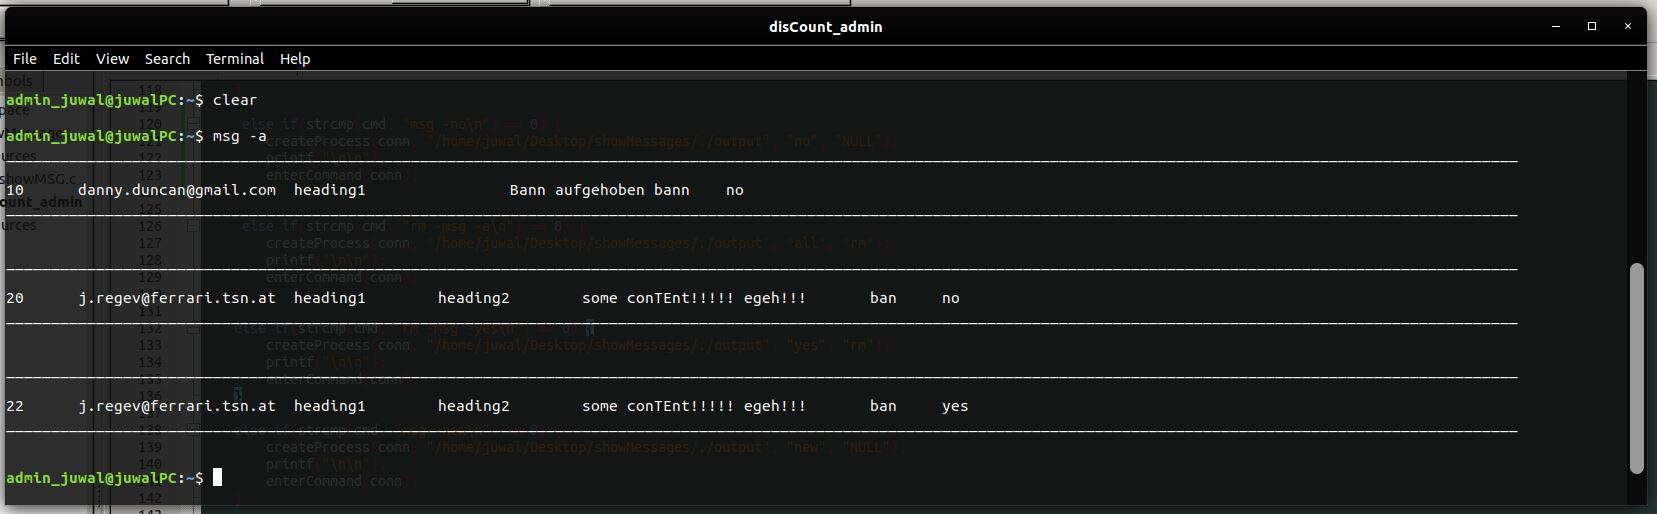
\includegraphics[width=15cm]{images/msg_a}
	\caption[Befehl msg -a]{Ergebnis des Befehls msg -a}
\end{figure}
  
  

\subsubsection{msg -no}
Dieser Befehl zeigt alle noch ausständigen Nachrichten an.


\begin{figure}[b]
	\centering
	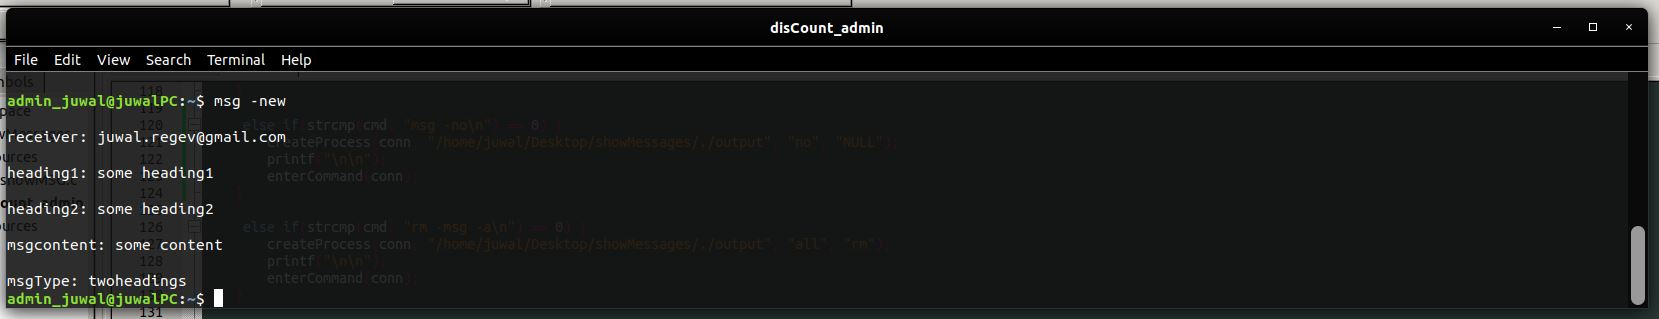
\includegraphics[width=15cm]{images/msg_new}
	\caption[Befehl msg -new]{Ergebnis des Befehls msg -new}
\end{figure}
  
\subsubsection{msg -new}
Hiermit kann man eine neue Nachricht verfassen und abrufbar machen.



\subsubsection{msg -yes}
Dieser Befehl zeigt alle bereits empfangenen Nachrichten an.



\subsubsection{rm -msg -yes}
Da bereits empfangene Nachrichten nutzlos sind und somit nur Platz verschwenden, können sie ganz einfach durch diesen Befehl gelöscht werden.

\subsubsection{rm -msg -all}
Damit können alle Nachrichten gelöscht werden.


\subsection{Sonstiges}

\subsubsection{clear und exit}
Wie im Linux-Terminal kann durch den ersteren Befehl das Terminal-Fenster aufgeräumt und durch den letzteren der Terminal verlassen werden. 


\chapter{Aufbau und Implementierung der Funktionen}

\subsection{Aufbau}
Das discount-Verwaltungsprogramm besteht aus drei Unterprogrammen: der Konsole, dem Redundanzenfinder und dem Nachrichtenfinder und Verfasser. Das Konsolen-Programm ordnet den eingegebenen Funktionen die richtigen Funktionen zu und ruft diese auch auf. Das Redundanzen-Programm sucht und löscht identische Lösungen und dekrementiert die hochgeladenen Lösungen. Das Nachrichten-Programm löscht bestimmte Nachrichten und kann auch neue erzeugen.

\subsection{Prozesserzeugung in Linux}
Da im Programm Systemaufrufe zum Erzeugen von Prozessen verwendet werden, werden diese nun kurz vorgestellt.

\subsubsection{fork()}
,,fork() ist der einzige Weg in Linux einen neuen Prozess zu erzeugen. Der Systemaufruf erzeugt eine exakte Kopie des Aufruferprozesses, einschließlich des CPU-Zustandes (Register, Programmzählers, ...). Diese Kopie wird zum Kindprozess. Vaterprozess und Kindprozess laufen jetzt unabhängig voneinander, haben jedoch die exakt selben Daten im Adressraum. Der fork-Systemaufruf gibt dem Vaterprozess den Prozess-Identifikator des Kindprozesses, welcher größer als null ist und dem Kindprozess null zurück. Durch diese Rückgabewerte lässt sich unterscheiden,welcher der Vater -und welcher der Kindprozess ist. Somit können diese auch unterschiedlichen Code ausführen.'' (vgl. Tanenbaum 2009, S. 50 ff.\nocite{OS})

\subsubsection{exec()}
,,Dieser Systemaufruf lädt ein neues Programm in den Adressraum des Prozesses. Das Programm kann mithilfe dessen Pfad als Parameter übergeben werden.'' (vgl. ebda. S. 52f. \nocite{OS})

\subsubsection{wait()}
,,Dieser Systemaufruf zwingt den Aufruferprozess auf das Terminieren seiner Kindprozesse zu warten.'' (vgl. ebda. S. 52 \nocite{OS})

\subsection{Implementierung}

\subsubsection{Konsolenprogramm}

\begin{lstlisting}
void enterCommand(MYSQL *conn)
\end{lstlisting}

\noindent Zu allererst wird mit dieser Funktion eine Verbindung zur Datenbank aufgestellt. Ist dieser Schritt erfolgreich, wird folgende Funktion aufgerufen:\\



\begin{lstlisting}
else if(strcmp(cmd, "rm -hbla -a\n") == 0) {
        createProcess(conn, "/home/juwal/Desktop/showDuplicates/./output", "usersolutionshbla4", "rm");
        printf("\n\n");
        enterCommand(conn);
}
\end{lstlisting}

\noindent Der eingegebene Befehl des Benutzers wird in einem Pointer gespeichert und durch eine Reihe von if-Statements mit den verfügbaren Befehlen verglichen. Ein Vergleich könnte wie oben gezeigt aussehen.\\



\begin{lstlisting}
void createProcess(MYSQL* conn, char* path, char* table, char* extraOp) {

    int ret = fork();           //neuen Prozess erstellen

    if(ret == -1)
        exit(-1);
    

 //fork() gibt dem Kindprozess 0 zurueck

    else if(ret == 0)
        execv(path, (char *[]){(char*) table, (char*) extraOp, NULL});       //ladet ein neues Programm


    //ret > 0, deshalb hier Vaterprozess

    else {
        wait();      //wartet bis Kindprozess terminiert
        enterCommand(conn);
    }

}
\end{lstlisting}

\noindent Da das Redundanzenprogramm ein selbstständiges Programm ist, wird für dieses in der Funktion createProcess ein neuer Prozess erzeugt.\\
So wird mit fork() der Kindprozess erstellt. Gibt dieser Systemaufruf -1 zurück, konnte der Prozess nicht erfolgreich erzeugt werden und das Programm terminiert. Wird null zurückgegeben, handelt es sich um den Kindprozess und wir laden ein neues Programm in dessen Adressraum. Als Parameter für dessen main-Funktion, geben wir noch den Namen der Tabelle, in welcher eine Operation ausgeführt werden soll und eine Extraoperation wie zum Beispiel ,,rm'' für das Löschen bestimmter Datensätze, mit. Ist ret größer als null handelt es sich um den Vaterprozess, also der Konsole, welche vorerst durch wait() auf das Terminieren aller Kindprozesse warten muss und dann durch den Aufruf von ,,enterCommand()'' wieder für den nächsten Befehl bereit ist.\\

\subsubsection{Programm zum Anzeigen und Löschen von Redundanzen}
Als nächstes widmen wir uns dem Programm zum Anzeigen und Löschen der Redundanzen. In dessen main-Funktion wird wieder eine Verbindung zur Datenbank aufgebaut und bei Erfolg die Funktion ,,showDuplicates(conn, argv[0])'' aufgerufen, wobei argv[0] auf die Tabelle zeigt, dessen Dubletten angezeigt werden sollen. Wir werden hier nur auf die wichtigsten Bestandteile eingehen:\\


\begin{lstlisting}
    char tempQuery[50];
    sprintf(tempQuery, "SELECT code FROM %s", table);
    mysql_query(conn, tempQuery);
    res = mysql_store_result(conn);
\end{lstlisting}

\noindent Die SQL-Abfrage holt alle Lösungen aus der Tabelle und speichert sie in res.\\

\begin{lstlisting}
    int totalRowCount = mysql_num_rows(res);
    char *code[totalRowCount];
\end{lstlisting}

\noindent Anschließend werden in der Variablen totalRowCount die Anzahl der geholten Lösungen gespeichert, welche für die Initialisierung des code-Arrays verwendet wird.\\

\begin{lstlisting}
    int i = 0;
    while(row = mysql_fetch_row(res)) {

        code[i] = (char*) row[0];
        i++;

    }
\end{lstlisting}


\noindent In diesen Array werden dann alle Adressen der Lösungen gespeichert.\\

\begin{lstlisting}
    char query[1000];
    
    static int duplicatesID[1000] = {-1};   //dieser Array wird von showDuplicates zurueckgegeben
    
    char *duplicates[totalRowCount];     //hier wird der Code der Duplikate gespeichert
    
    int j = 0;   //zeigt die naechste freie Stelle im duplicatesID-Array an
    
    i = 0;       //zeigt die naechste freie Stelle im duplicates-Array an

\end{lstlisting}

\noindent Es folgen einige Initialisierungen, dessen Funktion in Kommentarform daneben steht. Im duplicatesID-Array werden alle ID's der Redundanzen gespeichert, damit eine später eingeführte Funktionen diese in einer SQL-Abfrage zum Löschen der Datensätze verwenden kann.\\


\begin{lstlisting}
    for(int rowIndex = 0; rowIndex < totalRowCount; rowIndex++) {

        for(int x = 0; x < i; x++) {

            if(strcmp(duplicates[x], code[rowIndex]) == 0)
                goto outer;

        }

        sprintf(query, "SELECT * FROM %s WHERE code=('%s')", school, code[rowIndex]);
        mysql_query(conn, query);
        res = mysql_store_result(conn);
\end{lstlisting}

\noindent Es wird nun durch alle Lösungen durchiteriert und durch eine SQL-Abfrage überprüft, ob diese irgendwo noch einmal vorkommen. Davor wird noch kontrolliert, ob die Lösung bereits als Redundanz gekennzeichnet wurde. Wenn ja, wird der Inhalt der for-Loop durch das goto-Statement übersprungen, damit die Redundanzen nicht doppelt ausgegeben werden.\\
Alle bei der SQL-Abfrage gefundenen Dubletten werden in res gespeichert und später weiter verarbeitet.\\




\begin{lstlisting}
        int rowCount = mysql_num_rows(res);
\end{lstlisting}

\noindent Die Anzahl der identischen Datensätze wird in rowCount gespeichert.\\


\begin{lstlisting}
        if(rowCount > 1) {

            duplicates[i] = (char*) code[rowIndex];
            i++;
\end{lstlisting}

\noindent Wenn mehr als ein identischer Datensatz gefunden wurde, gibt es mindestens ein Duplikat und es muss etwas ausgegeben werden. Im den duplicates-Array wird der redundante Inhalt eingetragen.\\

\begin{lstlisting}
    printf("\n\n%i occurences in database\n", rowCount);
    printf("___________________________\n");

    while(row = mysql_fetch_row(res)) {

        duplicatesID[j] = convertToInt(row[0]);           //jede ID der Duplikate in das Array eintragen
        j++;
        printf("\n%s\t%s\t%s\t%s\t%s\t%s\t%s", row[0], row[1], row[2], row[3], row[4], row[5], row[6]);

    }

    printf("\n_______________________\n\n\n");
\end{lstlisting}

\noindent Die kommpletten Informationen der Redundanzen werden ausgegeben und deren ID in den duplicatesID-Array eingetragen.\\


\begin{lstlisting}
            j--;
\end{lstlisting}

\noindent Da alle Duplikate mit Ausnahme von einem gelöscht werden sollen, wird der letzte Eintrag durch das Dekrementieren von j beim nächsten Mal überschrieben und somit gleichzeitig aus dem Array gelöscht.\\


\begin{lstlisting}
        }

    outer:
    ;

    }

    sizeDuplicatesID = j;
    return duplicatesID;
    
}
\end{lstlisting}

\noindent Zum Schluss wird noch die globale Variable sizeDuplicatesID mit der Größe des duplicatesID-Array gesetzt und dieser auch zurückgegeben.\\


\begin{lstlisting}
int *tempP = showDuplicates(conn, argv[0]);
\end{lstlisting}

\noindent Die showDuplicates-Funktion wurde von der main-Funktion aufgerufen und kehrt dort wieder mit der Adresse des showDuplicates-Array zurück, welche im Pointer tempP gespeichert wird. Mit diesen Informationen werden dann die reduceAdded -und deleteDuplicates-Funktionen, je nachdem ob an der zweiten Stelle des Arrays und Parameters argv der main-Funktion ,,rm'' steht, aufgerufen oder nicht aufgerufen.


\subsection{Nachrichtenprogramm}
Auf dieses Programm wird nicht weiter eingegangen.








\part{Tabellenkalkulation}

\chapter{Tabellen in JAVA}
\rhead{KAPITEL 10.  TABELLEN IN JAVA}

\section{Grundlagen}
Um eine Tabelle in JAVA zu erstellen, muss ein JTable-Object initialisiert werden. Dieses wird in einen ,,Wrapper'', dem DefaultTableModel, eingebettet. Dieses stellt mehrere hilfreiche Funktionen zur Verfügung. Anschließend müssen die Zeilen und Spalten, welche am Anfang angezeigt werden, definiert werden. Die Anzahl dieser kann jedoch zur Laufzeit mit Hilfe des DefaultTableModels geändert werden.

\subsection{Listener}
Wie bei allen anderen GUI-Elementen, gibt es auch hier eine breite Anzahl an Listener. Hier werden nur die im Programm verwendeten erklärt.

\subsubsection{MouseListener}
Dieser wartet darauf, dass eine Zelle angeklickt wird. Durch bereitgestellte Funktionen kann dann unter anderem der Index der durch die Interaktion nun markierten Zelle geholt werden.

\subsubsection{TableModelListener}
Dieser wird, wie der Name schon verrät, dem DefaultTableModel zugeordnet. Er stellt eine nützliche Methode namens ,,tableChanged'' zur Verfügung. Sollte sich der Inhalt einer Zelle ändern, wird dieser aktiv.

\section{Probleme mit dem JTable}
In JAVA hat fast jedes GUI-Element einen eigenen Objekttyp. Mit diesem kommen in der Regel spezialisierte Funktionen, die dem Programmierer enorm viel Arbeit abnehmen und in Sachen Effizienz sehr ausgeklügelt sind. Leider gibt es keinen eigenen Objekttyp für eine JTable-Zelle. Das erschwert die Programmierung um einiges. Das größte Problem ist, dass man die einzelnen Zellen nur durch Renderer ansprechen kann. Ohne diese wirken sich Formatierungen immer auf die gesamte Tabelle aus. Auch kann man die Zellen nicht in einer Liste speichern. Man muss also immer die Koordinaten abfragen und diese dann in einem Array abspeichern. Dann muss man sie wieder herausfiltern und nach dem Wert an dieser Position fragen. Dass kein Objekttyp existiert, heißt auch, dass man den Zellen keinen Listener zuordnen kann. Wieder muss dieser Schritt durch Umwege selbst programmiert werden. Wie man sieht, führt das zu einer unnötigen Komplizierung des Codes.

\subsection{Renderer}
Hier wird nur der TableCellRenderer diskutiert. Dieser muss einem JTable zugeordnet werden. Alle Methoden darin beziehen sich automatisch auf alle Zellen. Man kann also auch hier keine einzelne Zelle direkt ansprechen. Dazu müssen if-Statements eingebaut werden, die nur bestimmte Zeilen beziehungsweise Spaltenindizes zulassen. So kann annähernd erreicht werden, was man will. Der Renderer wird jedes Mal aufgerufen, wenn irgendein ,,Event'' in der Tabelle auftritt. Das bedeutet, dass er parallel zu den anderen Listener der Tabelle ausgeführt wird und es möglicherweise zu Widersprüchen kommen kann, die alle geregelt werden müssen. Durch die Reaktion auf jedes Event, wird er außerdem oft ungewollt ausgeführt. Das wird geregelt, indem der eigentlich angesprochene Listener, eine boolsche Variable setzt, die dann im Renderer erkannt wird und die Funktion zur frühzeitigen Terminierung zwingt.







\chapter{Unterschied zu anderen Programmen und implementierte Funktionen}
\rhead{KAPITEL 11.  UNTERSCHIED ZU ANDEREN PROGRAMMEN UND IMPLEMENTIERTE FUNKTIONEN}
 
\section{Unterschied}
Die Berechnung von komplizierteren Verfahren aus dem Rechnungswesen, wird durch die Möglichkeit zur Verwendung einer Tabellenkalkulation enorm vereinfacht. Wieder gibt es hier bereits viele Programme die auf das Rechnen in einer Tabelle spezialisiert sind. Jedem Computerbenutzer sollte das Office-Programm ,,Excel'' bekannt sein. Da dieses Programm aber hauptsächlich auf den Büroalltag abgestimmt ist und es deshalb keine speziellen Features und Befehle bezüglich dem Rechnungswesen gibt, kommt man damit nicht viel schneller zur Lösung als auf dem Papier.\\
Die Tabellenkalkulation, welche in disCount implementiert wurde, unterstützt alle relevanten tabellenkalkulatorischen Funktionen. Zudem gibt es spezielle Befehle, die dem User viele Berechnungsschritte ersparen und ein effizientes und übersichtliches Arbeiten ermöglichen.



\section{Funktionen}

\subsection{Arithmetische Operationen}



\subsubsection{Berechnung von arithmetischen Operationen in einer Zelle}
Dazu muss man nur zwei Zahlen durch ein unterstütztes arithmetisches Symbol: ,,+, -, *, /'' trennen. Nachdem man die Tab-Taste gedrückt hat, erscheint das Ergebnis in der Zelle. Um die richtige Zelle zu erwischen, wurde ein TableChangeListener implementiert. Dieser wartet darauf, dass sich der Inhalt einer Zelle ändert. Tritt dieser Fall ein, holt er durch eine Abfrage den Index der geänderten Reihe und Spalte. Durch eine weitere Abfrage wird der enthaltene Wert erhalten, der gleich auf arithmetische Operationen überprüft wird. Sind keine enthalten, wird eine andere Methode, die erst diskutiert wird, ausgeführt. Sonst werden aus dem Inhalt der Zelle die beiden Zahlen herausgefiltert und das Ergebnis berechnet und ausgegeben.


\subsubsection{Berechnung von arithmetischen Operationen zwischen verschiedenen Zellen}
Die Verknüpfung der Werte zweier Zellen, durch eine erlaubte Operation, muss durch ein ,,='' eingeleitet werden. Anschließend wird die erste Zelle angeklickt. Deren Wert erscheint dann nach dem ,,=''. Nun muss ein arithmetisches Zeichen eingegeben und anschließend die zweite Zelle ausgewählt werden. Deren Wert erscheint auch in der Zelle und nach dem Drücken der Tab-Taste, wird der Inhalt durch das Ergebnis ersetzt. Die Implementation dieser Funktion ist wesentlich komplexer als die obere, da jetzt mehrere Klicks des Users involviert sind. Da bei einem Klick auch der MouseListener ausgeführt wird, gibt es eine Kommunikation zwischen den beiden mit Hilfe von boolschen Variablen, die das Ausführen erlauben oder nicht. Wurde der Wert vollständig eingegeben, wird nun nach dem Vorhandensein des ,,=''-Zeichens geprüft. Ist es enthalten, wird es vom String gelöscht und die Tabelle aktualisiert. Der neue String wird nun von der Methode oben erkannt und der analoge Algorithmus wird ausgeführt.


\subsubsection{Berechnung des Produktes beziehungsweise der Summe durch das Markieren von Zellen}
In der Tabelle wird durch das Markieren von einer Zeile und zwei Spalten, das Produkt der darin enthaltenen Werte berechnet. Werden beliebig viele Zeilen und eine Spalte markiert, wird die Summe berechnet. Wird ein Zellbereich markiert und die Entertaste gedrückt, wird eine Methode aktiv, die eine weitere Methode aufruft, welche einen Array mit den Indizes der markierten Zeilen beziehungsweise Spalten zurückgibt. Nach der Analyse der Länge des Arrays, steht fest ob es sich um eine horizontale oder vertikale Operation handelt. Das weitere Verfahren wird im nächsten Abschnitt erklärt. 


\subsubsection{Erstellung von Abhängigkeiten, die auf Änderungen reagieren}
Nachdem die Art der Operation festgestellt wurde, werden die Indizes der in die Berechnung involvierten Zellen, zusammen in eine Liste eingetragen, die in eine Hauptliste eingebettet ist. Die Einträge gehören ab jetzt zusammen und sind von einander abhängig. Das heißt: wenn eine dieser Zellen verändert wird, wird erneut die Summe beziehungsweise das Produkt berechnet.

\subsubsection{Entstandenen Beziehungen werden durch Farben angezeigt}
Damit der Benutzer stets weiß, wie er zu einem Ergebnis gekommen ist, werden beim Klick auf eine Zelle, alle Zellen, die eine Beziehung zu der ausgewählten haben, in der gleichen Farbe umrahmt. Da es hier wieder Komplikationen mit dem Renderer gibt und der Algorithmus verhältnismäßig lang ist, wird nicht genauer auf diesen und den der obigen Funktion eingegangen.





\part{Speicherung und Dateiformat}

\chapter{Encodierung}
\rhead{KAPITEL 13.  ENCODIERUNG}
Wir wollen generell zwei Arten von Dateien speichern. Einmal die Textdatei mit den Buchungssätzen und einmal die disCount-Datei mit der Encodierung. Auf die Speicherung dieser beiden Dateien wird zuerst eingegangen.


\section{Übersicht über den Ablauf}
Will der Benutzer die Buchungssätze in einer Textdatei speichern, wird automatisch auch eine Datei mit der Dateiendung dc, für disCount, abgespeichert. Damit zu diesem Zeitpunkt nicht alle Buchungssätze auf einmal encodiert werden müssen, wird das in kleinen Schritten erledigt, nämlich jedes Mal, wenn der Buchungssatz auf dem Arbeitspanel ausgegeben wird. Dazu werden beim Start des Programms zwei Listen angelegt. In einer der beiden werden die Buchungssätze, bereits mit den Abständen und den Zeilenumbrüchen, die in der Textdatei dann sichtbar sein sollen, uncodiert abgespeichert. In der anderen werden der Inhalt mit Encodierung gespeichert, die nun definiert wird.

\section{Definition und Implementierung der Codierung}

\subsection{Definition}
\# $:=$ signisalisiert den Anfang eines neuen Buchungssatzes\\
+ $:=$ Buchungssatz hat rechts mehr Konten als links\\
- $:=$ umgekehrt\\
2 | 3 | 4 $:=$ die Anzahl der zu erwartenden Konten\\
* $:=$ signisalisiert den Anfang des ersten Kontos\\
/ $:=$ trennt die Konten und Beträge von einander\\
\& $:=$ signisalisiert den Anfang des ersten Betrages\\

\subsection{Implementierung}

\subsubsection{ohne Encodierung}
\begin{lstlisting}
MainModel.contentForTxt.addLast("\r\n\r\n\r\n\r\n" + konto1 + "    " + konto2);
MainModel.contentForTxt.addLast("\r\n" + konto3);

MainModel.contentForTxt.add(MainModel.contentForTxt.size()-1, "                " + round(price1) + "    " + round(price2));
MainModel.contentForTxt.addLast("                        " + round(price3));
\end{lstlisting}

\noindent Der obenstehende Code deckt die Fälle der zweistufigen Buchungssätze mit mehr Konten auf der linken Seite ab. Die anderen Fälle können von der Leserin oder dem Leser selbst nachvollzogen werden. Gleiches gilt für folgenden Code.\\

\subsubsection{mit Encodierung}
\begin{lstlisting}
MainModel.contentForTxt_load.addLast("#-3*" + konto1 + "/" + konto2 + "/" + konto3);

MainModel.contentForTxt_load.add("&" + round(price1) + "/" + round(price2) + "/" + round(price3));
\end{lstlisting}



\chapter{Decodierung}
\rhead{KAPITEL 14.  DECODIERUNG}
Dieser Part ist wesentlich anspruchsvoller als letzterer. Deswegen wird diesmal auch der entworfene Code erklärt.

\section{Vorbereitung}
Bevor wir uns den Code anschauen, sollte die Leserin oder der Leser wissen, dass die Buchungssätze in einen character-Array geladen werden, da bei der Entschlüsselung jedes einzelne Zeichen von größter Bedeutung ist.

\section{Umsetzung}

\begin{lstlisting}
private static void prepareCollection(int index) {
	
  boolean leftmore = false;
	
  if(index == -1)
     return;
	
  else {
		
     LinkedList<String> llKontos = new LinkedList<String>();
     LinkedList<String> llPrices = new LinkedList<String>();
		
     char currentChar = llChar.get(index);
     int kontoCount = 0;
		
     if(currentChar == '#') {
	   currentChar = llChar.get(++index);
			
	  if(currentChar == '-')
	      leftmore = true;
			
	  currentChar = llChar.get(++index);
			
	  kontoCount = Integer.parseInt(Character.toString(currentChar));
\end{lstlisting}

\noindent ,,leftmore'' signalisiert hier, dass der Buchungssatz mehr Konten auf der linken Seite enthält. Nachdem der Austrittsfall abgeklärt wurde, werden zwei Listen angelegt, in welchen später die herausgelesenen Konten beziehungsweise Beträge gespeichert werden. Die Variable ,,kontoCount'' wird später zur Unterscheidung der Buchungssatzarten verwendet. Es wird dann Schritt für Schritt überprüft, ob die Eingabe passt und kontoCount wird gesetzt. Dann folgt diese Zeile:

\begin{lstlisting}
index = collectKontos_Prices(llPrices, collectKontos_Prices(llKontos, ++index));
\end{lstlisting}

\noindent Sie ruft zweimal eine Methode auf, die die Liste weiter entschlüsselt. Als Argument geben wir dabei eine Liste mit, in welche die Konten beziehungsweise Beträge gespeichert werden sollen.

\begin{lstlisting}
private static int collectKontos_Prices(LinkedList<String> llKontos_Prices, int currentIndex_arg) {
		
  String konto = "";
  llKontos_Prices.addLast("");
		
  for(int currentIndex = ++currentIndex_arg; currentIndex < llChar.size(); currentIndex++) {
	char currentChar = llChar.get(currentIndex);
			
	if(currentChar == '/')
	   return collectKontos_Prices(llKontos_Prices, currentIndex);
\end{lstlisting}
\noindent Aus bestimmten Gründen wird am Anfang ein leerer Eintrag eingefügt. In einer for-Schleife wird dann auf ein ,,/''-Zeichen gewartet. Bei einem Treffer folgt dann ein rekursiver Aufruf. Für diesen wird dann die else-Variante der Funktion interessant, die so lautet:

\begin{lstlisting}
  else {
				
     if(currentChar == '&' || currentChar == '#' || currentChar == -1) {
        return currentIndex;
     }
				
     else {
        konto = konto + Character.toString(currentChar);
        llKontos_Prices.set(llKontos_Prices.size() - 1, konto);
     }
  }
 }
		
 return -1;
}
\end{lstlisting}
\noindent \& beziehungsweise \# beziehungsweise -1 bedeuten den Anfang der Beträge beziehungsweise den Anfang eines neuen Buchungssatzes beziehungsweise das Ende der Liste und deshalb ist die Konsequenz die Rückgabe der Methode mit dem aktuellen Index. Bei der ersten Rückgabe, wird die Methode von der Aufrufermethode erneut mit dem aktuellen Index und der Liste der Beträge aufgerufen. Die Aufgabe ist nun die Beträge herauszufiltern und mit diesen die Liste zu füllen.\\

\noindent Ansonsten ist das Zeichen eine Konto beziehungsweise Betragnummer und deshalb wird sie dem angefangenen Konto beziehungsweise Betrag und anschließend der Liste hinzugefügt. Das wird so lange gemacht, bis die anderen Fälle wieder eintreten. Angenommen es trit nun der Fall ,,-1'' beziehungsweise ,,\#'' ein. Das heißt, dass nun das Ende der Liste erreicht ist beziehungsweise ein Buchungssatz vollständig abgeschlossen ist, also bereits Kontonummern und Beträge vollständig in den Listen sind und diese wiederum bereit zur Verarbeitung sind.


\begin{lstlisting}
  if(kontoCount == 2) {
      Basic_Model.paint2Konten(llKontos.get(0), llKontos.get(1));
      MainModel.paint1Price(Double.parseDouble(llPrices.get(0)));
  }

  else if(kontoCount == 4){
      Basic_Model.paint4Konten(llKontos.get(0), llKontos.get(1), llKontos.get(2), llKontos.get(3));
      MainModel.paint4Prices(Double.parseDouble(llPrices.get(0)),  Double.parseDouble(llPrices.get(1)), Double.parseDouble(llPrices.get(2)), Double.parseDouble(llPrices.get(3)));
  }

  else if(kontoCount == 3 && leftmore == true) {
      Basic_Model.paint3Konten(llKontos.get(0), llKontos.get(1), llKontos.get(2));
      MainModel.paint3Prices(Double.parseDouble(llPrices.get(0)),  Double.parseDouble(llPrices.get(1)), Double.parseDouble(llPrices.get(2)));
  }

  else {
      View_SuperClass.swapLeft_RightWP();
      Basic_Model.paint3Konten(llKontos.get(1), llKontos.get(0), llKontos.get(2));
      MainModel.paint3Prices(Double.parseDouble(llPrices.get(1)),  Double.parseDouble(llPrices.get(0)), Double.parseDouble(llPrices.get(2)));
      View_SuperClass.resetSwap();
  }
  prepareCollection(index);
 }	
}
\end{lstlisting}
\noindent Es wird nun, auf Basis des Inhalts von kontoCount, entschieden, welche Routine zum Ausgeben der Buchungssätze gewählt werden soll. Diese Routinen sind selbsterklärend. Erklärungsbedarf hat möglicherweise der rekursive Aufruf in der letzten Code-Zeile: Die Funktion ist ja oben zurückgekehrt, weil ein Buchungssatz vollständig decodiert wurde. Es können natürlich noch weitere folgen, bei denen dann wieder von vorne begonnen werden muss und deshalb wird die Funktion erneut aufgerufen.

\begin{lstlisting}
\end{lstlisting}
\newpage




\section*{Zusammenfassung} 
\addcontentsline{toc}{part}{Zusammenfassung} 
\rhead{}
 
In disCount wurden einige objektorientierte Konzepte implementiert. Dazu gehören die Vererbung und das MVC-Pattern. Letzteres wurde in einer etwas modifizierten Art umgesetzt. Die Benutzeroberfläche ist in mehrere Hauptarbeitsflächen gegliedert und darauf ausgelegt, auch kleinere Bildschirmauflösungen zu unterstützen. Es wurden Methoden zur Darstellung von verschiedenen Buchungssatzarten entwickelt. Auf einen Ausnahmefall, die Abschreibung, wird besonders eingegangen. Eine weitere wichtige Funktion ist die Angabenanalyse, die eine Angabe als Input nimmt und daraus mithilfe von eigenen Methoden, die richtigen Buchungssätze erstellt. Diese Funktion ist jedoch erst für ein Themengebiet verfügbar. Mit der Lösungsvorschläge-Funktion können Schülerinnen und Schüler fertige Lösungen auf eine Datenbank hochladen. Einer anderen Benutzerin oder einem anderen Benutzer werden diese Lösungen bei teilweiser Übereinstimmung vorgeschlagen. Die Benutzerin oder der Benutzer kann den Lösungsvorschlag mit einem Daumen hoch oder runter bewerten. Die Fehlerkorrektur kontrolliert die zur Evaluation freigegebene Aufgabe und weist auch auf die Art des Fehlers hin. Zu determinieren, ob nun ein Buchungssatz zu viel oder zu wenig ist oder ob er einfach nur fehlerhaft ist, stellt eine Herausforderung dar. Die Tabellenkalkulation in disCount ist in der Lage Berechnungen durch Eingabe von Befehlen durchzuführen. Um Befehle auf ihre Richtigkeit zu überprüfen, wurde eine Grammatik entwickelt. Damit Schülerinnen und Schüler ihre Arbeit exportieren und importieren können, benötigt es ein eigenes Dateiformat. Buchungssätze werden beim Export in das eigens entwickelte Dateiformat ,,dc'' encodiert und beim Import wieder decodiert.

\bibliographystyle{plain}
\bibliography{literatur}
\addcontentsline{toc}{part}{Literaturverzeichnis}


\listoffigures
\addcontentsline{toc}{part}{Abbildungsverzeichnis}

\newpage
\newpage


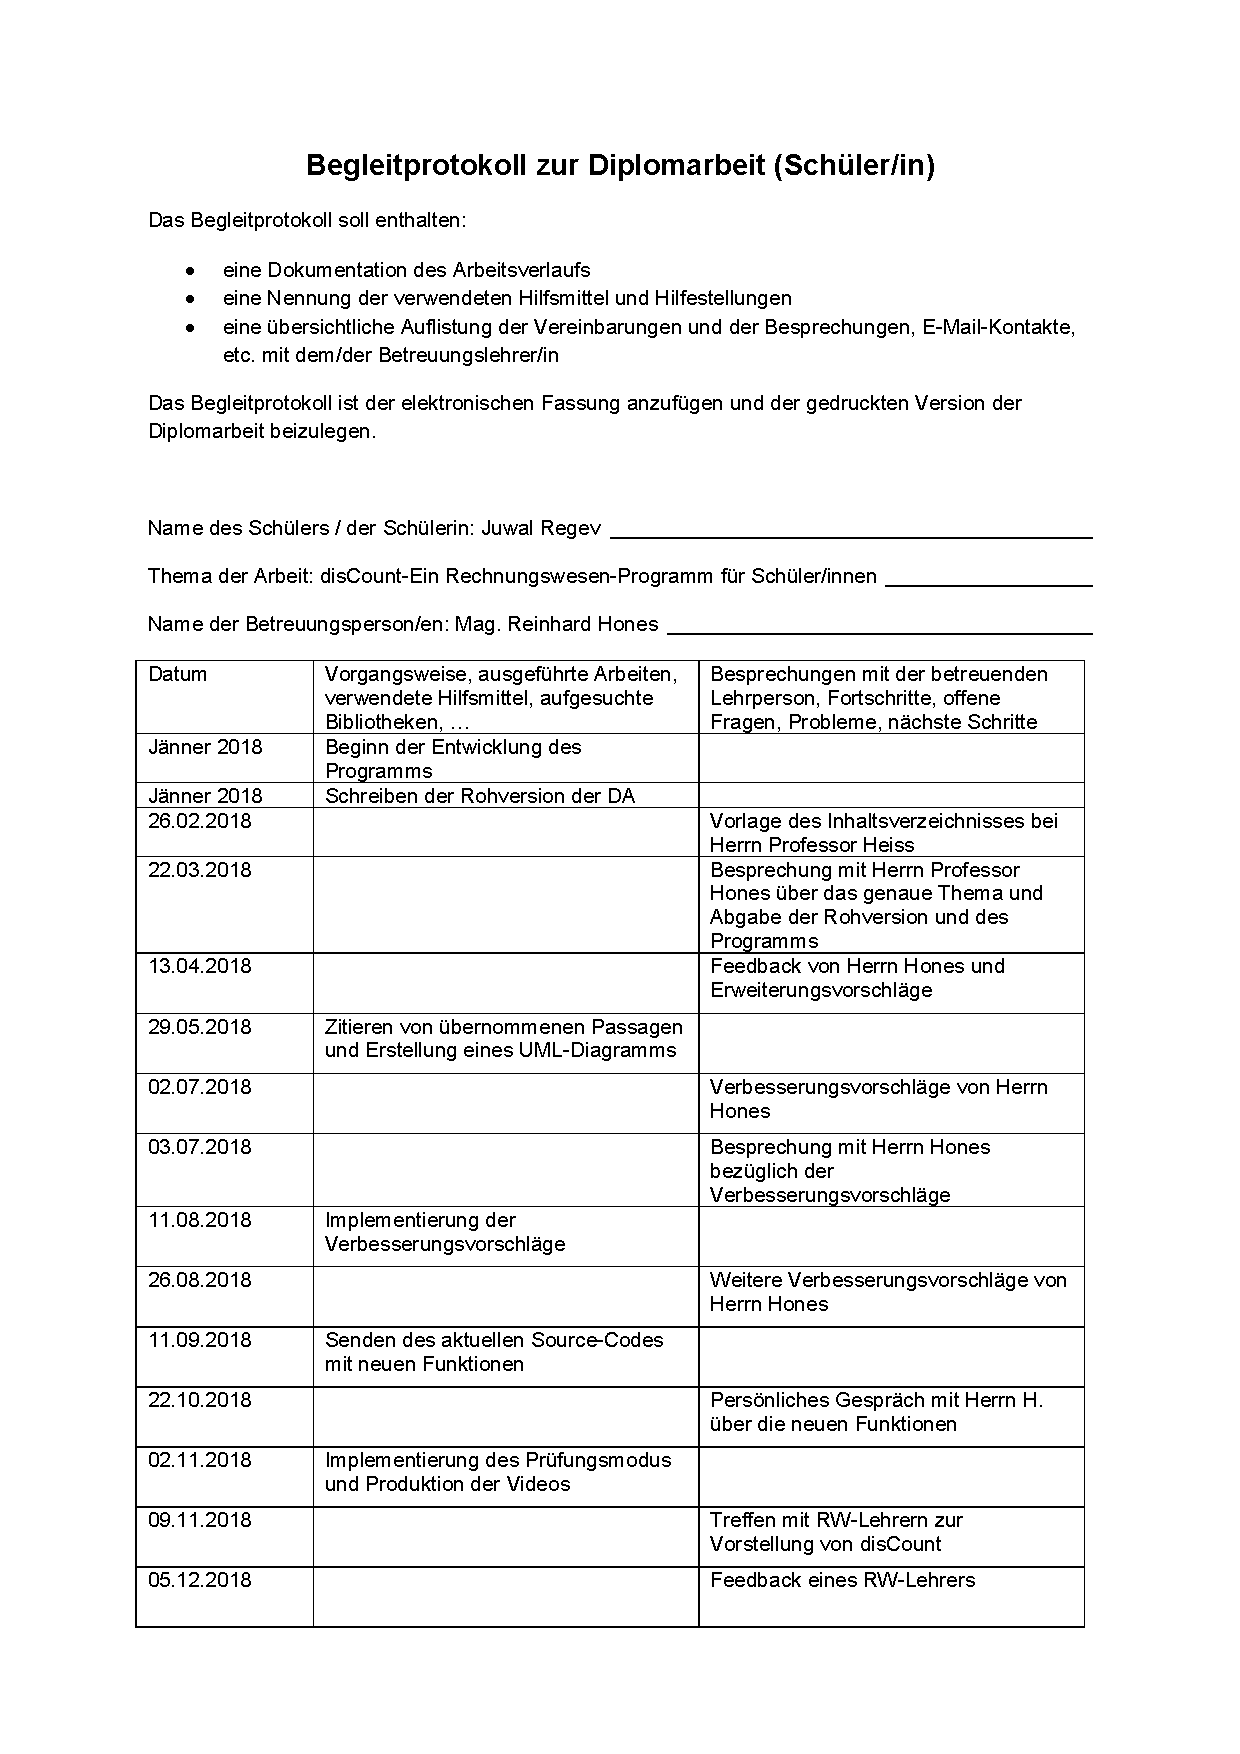
\includepdf[pages=-]{images/begleitprotokoll}


\appendix
\addcontentsline{toc}{part}{Anhang}						
\chapter{MVC-Umsetzung in disCount}

\begin{figure}[h]
	\centering
	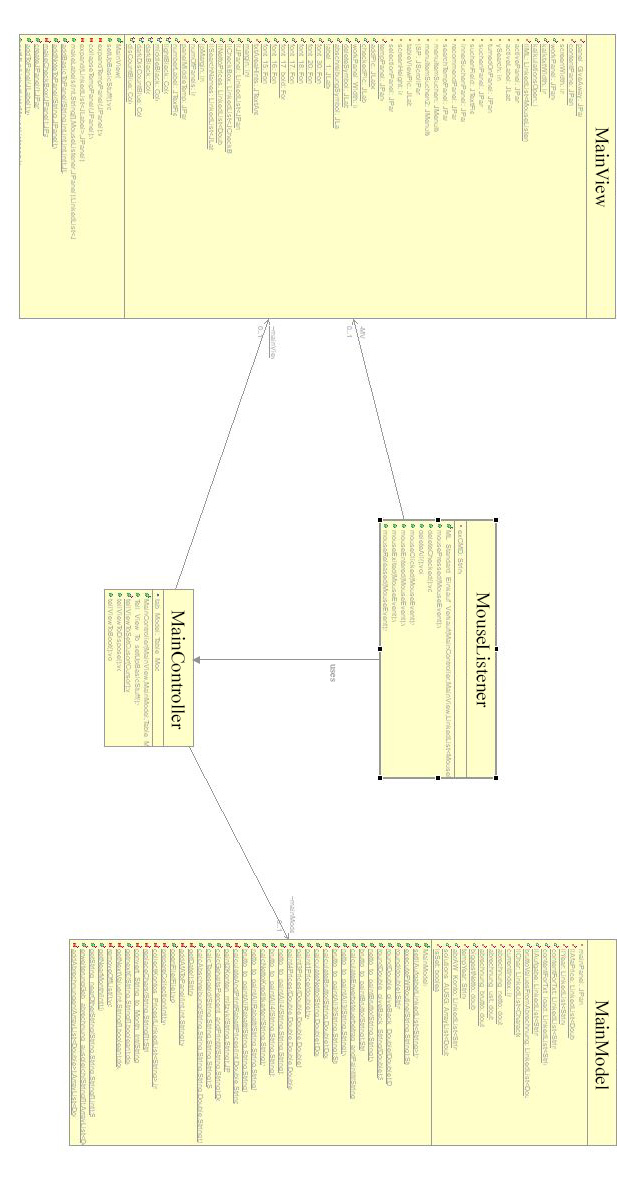
\includegraphics[height=18cm]{images/mvc_dc}
\end{figure}


\end{document}